\section{离散时间信号的傅里叶分析}

实际信号在时域上一般是连续的,而且持续时间通常较长;
在频域上,实际信号的频谱也是连续的。但是,数字处理设备(例如计算机)
只能存储有限多的数据,只能表示有限多的数值。因此,我们需要对信号
进行离散化处理,将较长的持续时间转化为有限长时间范围内离散的时间点,
同时,将连续的信号取值限制在一定范围、一定精度内。这样,我们就得到了离散时间信号。

这就是我们在本章要讨论的内容:离散时间信号的傅里叶分析。

% \subsection{面临的矛盾与问题}

\subsubsection{矛盾 1:如何在信号信息不受损的情况下对时域信号进行离散化?}

我们可以考虑对信号在时域上进行理想采样,也就是说,采样过程需要满足采样定理,
则可以保证在信息不受损的情况下对信号进行离散化:

\begin{enumerate}[label=(\arabic*)]
    \item 信号频带宽度有限,例如限制在 $[-\omega_M, \omega_M]$ 内。
    \item 采样频率满足 $\omega_s \ge 2\omega_M$。
\end{enumerate}

至此,矛盾 1 已解决。

\subsubsection{矛盾 2:如何从采样信号的频谱恢复出原信号的频谱?}

我们可以在时域上进行带限内插,从采样信号中恢复出原信号。
理论上只要在采样时满足采样定理,即可恢复出原信号的频谱。
但实际工程中,采样频率必须满足 $\omega_s > 2\omega_M$,
即\bd{严格大于}采样定理中的条件,才能保证内插还原的信号与原信号一致。

至此,矛盾 2 已解决。

\subsubsection{矛盾 3:如何计算采样信号的频谱?}

对于连续信号,我们可以直接使用傅里叶变换计算其频谱。
但对于\bd{没有解析式}的信号(例如某些实际观测到的信号),
无法通过解析式得到信号的连续频谱。

采样信号是离散的,我们该如何计算出采样信号的频谱呢?

\subsubsection{矛盾 4:在截取某一段信号进行频谱分析时,信号的频谱与原频谱相比会发生什么变化?}

在实际工程中,我们往往只能获取信号的有限长片段,而不是整个信号,
这是因为信号的持续时间往往会超出设备的处理能力。

\begin{enumerate}[label=(\arabic*)]
    \item 截取信号会不会影响对信号的分析?
    \item 截取信号得到的频谱与原频谱相比会发生什么变化?
\end{enumerate}

\subsubsection{矛盾 5:如何存储离散信号的频谱?如何从有限的离散频谱中恢复出采样信号?}

离散信号的频谱是连续的周期函数,所以我们可以
\begin{enumerate}[label=(\arabic*)]
    \item 存储有限长度的频谱(有限范围),可以只保存一个周期的频谱信息。
    \item 存储有限数目的频谱(有限数目),可以只存离散频率处的频谱值。
\end{enumerate}

后者本质上是对连续周期频谱中的某一周期的采样。由于函数在一个周期内必然是带限的,
因此如果按照满足采样定理的条件来采样,则可以通过插值方法恢复出原离散信号。

\subsubsection{矛盾 6:如何实现离散信号与离散频谱之间的快速计算?}

如果按照定义来实现离散信号的离散时间傅里叶变换,那么计算量将会非常大,
难以推广到实际应用中。因此,我们需要寻找一种快速计算的方法。

这包含两个问题:
\begin{enumerate}[label=(\arabic*)]
    \item 如何由离散信号计算出离散频谱?
    \item 如何由离散频谱计算出离散信号?
\end{enumerate}

% \subsection{离散时间傅里叶变换}

\subsubsection{采样信号与采样频谱}

对于采样信号
\begin{align*}
    \hat{f}(t) = \sum_{n = -\infty}^{+\infty}f(nT_s)\delta(t - nT_s),
\end{align*}
以及其频谱函数
\begin{align*}
    \hat{F}(\omega) = \frac{1}{T_s}\sum_{k = -\infty}^{+\infty}F(\omega - k\omega_s),
\end{align*}
而言,如果采样过程满足采样定理的要求,则在奈奎斯特区间内,以下等式成立:
\begin{align*}
    T\hat{F}(\omega) = F(\omega), \quad \omega \in \left[-\frac{\omega_s}{2}, \frac{\omega_s}{2}\right].
\end{align*}
如果采样过程不满足采样定理的要求,则会发生混叠,在 $[-\omega_s/2, \omega_s/2]$ 这个
区间内混有其他部分``扩展''过来的密度分布。此时
\begin{align*}
    T\hat{F}(\omega) = F(\omega) + F(\omega - \omega_s) + F(\omega + \omega_s) + \cdots,
\end{align*}
我们可以认为,$F(\omega) \approx T\hat{F}(\omega)$。

\begin{theorem}
    对于连续时间信号 $f(t)$ 进行以 $T_s$ 为时间间隔的采样,得到序列 $f(nT_s)$,
    其中 $n \in \set{Z}$。那么,
    \begin{align*}
        \hat{F}(\omega) = \sum_{n = -\infty}^{+\infty}f(nT_s)\mathe^{-\mathi\omega nT_s}.
    \end{align*}
    这说明仅使用采样值 $f(nT_s)$ 即可计算出理想采样信号的频谱密度函数。
    注意,此时的频谱密度函数 $\hat{F}(\omega)$ 是连续的,且为周期函数。
\end{theorem}

\begin{theorem}
    若将 DTFT 看做是对 $\hat{F}(\omega)$ 的傅里叶展开,则 $f(nT_s)$ 即为
    $\hat{F}(\omega)$ 的傅里叶系数。因此,
    \begin{align*}
        f(nT_s) = \frac{1}{\omega_s}\int_{-\omega_s/2}^{\omega_s/2}\hat{F}(\omega)\mathe^{\mathi\omega nT_s}\D{\omega}.
    \end{align*}
\end{theorem}

\subsubsection{数字信号与数字频谱}

由于采样间隔为固定的值,因此不妨设 $T_s = 1$,这就是在对 DTFT 进行
频率归一化(采样间隔归一化等价于频率归一化,因为二者是互为倒数的)。
这样,具体的物理时间被抽象为了数字信号中一个无量纲的``单位时间''。

\begin{definition}[离散时间傅里叶变换]
    我们称时间间隔归一的离散信号序列为\bd{数字信号},
    称其 DTFT 频谱函数为\bd{数字频谱}。
    设 $x(n)$ 为数字信号,其\bd{离散时间傅里叶变换}(DTFT)为 $X(\omega)$,则
    \begin{align*}
        X(\omega) & = \DTFT{x(n)} = \sum_{n = -\infty}^{+\infty}x(n)\mathe^{-\mathi\omega n}.
    \end{align*}
    反之,若已知 $X(\omega)$,则可以通过\bd{逆离散时间傅里叶变换}(IDTFT)求得 $x(n)$:
    \begin{align*}
        x(n) & = \IDTFT{X(\omega)} = \frac{1}{2\pi}\int_{-\pi}^{\pi}X(\omega)\mathe^{\mathi\omega n}\D{\omega}.
    \end{align*}
\end{definition}

\begin{remark}
    对于实际信号(模拟信号)而言,CTFT 中得到的是模拟频率 $\Omega$。
    在 DTFT 引入归一化时间后,变换结果是数字频率 $\omega$。
    模拟频率的奈奎斯特区间是
    \begin{align*}
        \left[-\frac{\Omega_s}{2}, \frac{\Omega_s}{2}\right],
    \end{align*}
    其中 $\Omega_s = 2\pi/T_s$,而数字频率的奈奎斯特区间是 $[-\pi, \pi]$。

    数字频率和模拟频率之间的关系是
    \begin{align*}
        \omega = \Omega \cdot \frac{2\pi}{\Omega_s} = \Omega \cdot T_s = \frac{\Omega}{f_s}.
    \end{align*}
    即数字频率是模拟频率的 $1/f_s$ 倍。这可以看做是将 $\Omega$ 的取值范围
    从 $[-\Omega_s/2, \Omega_s/2]$ 缩放到 $[-\pi, \pi]$。
\end{remark}

\begin{remark}
    进行频率归一化有以下好处:
    \begin{enumerate}[label=(\arabic*)]
        \item 频谱函数主周期内的形状,如果不考虑高低变化的话,
            则形状与采样间隔无关。
        \item 采样频率归一化使频谱重复间隔也会统一成 $2\pi$。
            考虑到离散信号频谱总是周期的函数,所以研究时可以对
            采样信号的实际频谱的周期进行抽象化的处理。抽象为 $2\pi$ 是很方便的。
        \item 在计算机程序中,计算过程可以只考虑数值表示,而不用考虑信号样本间的
            真实时间间隔。从算法效果上看,这不仅不会影响结果的正确性,
            反而还会提高算法应用的方便性。
    \end{enumerate}
\end{remark}

\begin{exercise}
    已知 $f(t)$ 的频谱函数为 $F(\omega)$,试证明:
    \begin{align*}
        T \cdot \sum_{n = -\infty}^{+\infty}f(nT_s) = \sum_{k = -\infty}^{+\infty}F(k\omega_s),
    \end{align*}
    其中 $\omega_s = 2\pi / T_s$。
\end{exercise}

\begin{proof}
    由于
    \begin{align*}
        \hat{F}(\omega) = \frac{1}{T_s}\sum_{m = -\infty}^{+\infty}F(\omega - m\omega_s),
    \end{align*}
    且
    \begin{align*}
        \hat{F}(\omega) = \sum_{n = -\infty}^{+\infty}f(nT_s)\mathe^{-\mathi\omega nT_s},
    \end{align*}
    故当 $\omega = 0$ 时,有
    \begin{align*}
        \frac{1}{T_s}\sum_{m = -\infty}^{+\infty}F(-m\omega_s) & = \hat{F}(0) \\
        & = \sum_{n = -\infty}^{+\infty}f(nT_s) \cdot \mathe^{0} \\
        & = \sum_{n = -\infty}^{+\infty}f(nT_s).
    \end{align*}
    此即
    \begin{align*}
        T_s \cdot \sum_{n = -\infty}^{+\infty}f(nT_s) = \sum_{m = -\infty}^{+\infty}F(-m\omega_s).
    \end{align*}
    命题得证。
\end{proof}

\subsubsection{离散时间傅里叶变换的性质}

\begin{property}[DTFT 的周期性]
    设 $x(n)$ 的 DTFT 为 $X(\omega)$,则有
    \begin{align*}
        X(\omega + 2\pi) = X(\omega).
    \end{align*}
\end{property}

\begin{property}[DTFT 是线性变换]
    设有 $k$ 个信号 $x_1(n), x_2(n), \cdots, x_k(n)$,则有
    \begin{align*}
        \DTFT{\sum_{i = 1}^{k}a_i x_i(n)} = \sum_{i = 1}^{k}a_i \DTFT{x_i(n)}.
    \end{align*}
    也就是说,信号线性组合的 DTFT,等于各信号的 DTFT 的线性组合。
\end{property}

\begin{property}[DTFT 的时移、频移性质]
    设 $x(n)$ 的 DTFT 为 $X(\omega)$,则有
    \begin{align*}
        \DTFT{x(n - n_0)} & = \mathe^{-\mathi\omega n_0}X(\omega), \\
        \DTFT{\mathe^{\mathi\omega_0 n}x(n)} & = X(\omega - \omega_0).
    \end{align*}
\end{property}

\begin{property}[DTFT 的反褶、共轭性质]
    设 $x(n)$ 的 DTFT 为 $X(\omega)$,则有
    \begin{align*}
        \DTFT{x(-n)} = X(-\omega), \quad \DTFT{x^*(n)} = X^*(-\omega).
    \end{align*}
\end{property}

\begin{exercise}
    已知 $x(n)$ 的 DTFT 为 $X(\omega)$,试求下列各序列的 DTFT:
    \begin{enumerate}[label=(\arabic*)]
        \item $x(n) * x^*(-n)$
        \item $x(n) - x(n + 2)$
        \item $x(n) * x(n + 1)$
    \end{enumerate}
\end{exercise}

\begin{solution}
    \begin{enumerate}[label=(\arabic*)]
        \item $\DTFT{x(n) * x^*(-n)} = \DTFT{x(n)} \cdot \DTFT{x^*(-n)}
            = X(\omega) \cdot X^*(\omega)$
        \item $\DTFT{x(n) - x(n + 2)} = \DTFT{x(n)} - \DTFT{x(n + 2)}
            = X(\omega) - \mathe^{2\mathi\omega}X(\omega)
            = (1 - \mathe^{2\mathi\omega})X(\omega)$
        \item $\DTFT{x(n) * x(n + 1)} = \DTFT{x(n)} \cdot \DTFT{x(n + 1)}
            = X(\omega) \cdot \mathe^{\mathi\omega}X(\omega)
            = \mathe^{\mathi\omega}(X(\omega))^2$
    \end{enumerate}
\end{solution}

\begin{property}[DTFT 的时域扩展性质]
    设 $x(n)$ 的 DTFT 为 $X(\omega)$,则有
    \begin{align*}
        x_{(a)}(n) = \begin{cases}
            x(n/a), & n/a \in \set{Z}, \\
            0, & \text{otherwise},
        \end{cases}
    \end{align*}
    其中 $a \in \set{Z}$ 且 $a \neq 0$。对应地,有
    \begin{align*}
        \DTFT{x_{(a)}(n)} = X(a\omega).
    \end{align*}
\end{property}

\begin{exercise}
    证明:若 $X(\omega)$ 是 $x(n)$ 的 DTFT,则
    \begin{align*}
        y(n) = \begin{cases}
            x(n / L), & n = 0, \pm L, \pm 2L, \cdots, \\
            0, & \text{otherwise},
        \end{cases}
    \end{align*}
    的 DTFT $Y(\omega)$ 满足 $Y(\omega) = X(L \omega)$。
\end{exercise}

\begin{proof}
    由题知,对于 $k \in \set{Z}$,都有 $y(kL) = x(k)$。因此,
    \begin{align*}
        Y(\omega) & = \sum_{n = -\infty}^{+\infty}y(n)\mathe^{-\mathi\omega n} \\
        & = \sum_{k = -\infty}^{+\infty}y(k L)\mathe^{-\mathi\omega kL} \\
        & = \sum_{k = -\infty}^{+\infty}x(k)\mathe^{-\mathi\omega kL} \\
        & = X(L\omega).
    \end{align*}
    命题得证。
\end{proof}

\begin{property}[DTFT 的频域微分性质]
    设 $x(n)$ 的 DTFT 为 $X(\omega)$,则有
    \begin{align*}
        \DTFT{n x(n)} = \mathi\frac{\D{X(\omega)}}{\D{\omega}}.
    \end{align*}
\end{property}

\begin{property}[DTFT 的时域卷积定理]
    设 $x_1(n)$ 和 $x_2(n)$ 的 DTFT 分别为 $X_1(\omega)$ 和 $X_2(\omega)$,则有
    \begin{align*}
        \DTFT{x_1(n) * x_2(n)} = X_1(\omega)X_2(\omega).
    \end{align*}
\end{property}

\begin{property}[DTFT 的频域卷积定理]
    设 $x_1(n)$ 和 $x_2(n)$ 的 DTFT 分别为 $X_1(\omega)$ 和 $X_2(\omega)$,则有
    \begin{align*}
        \DTFT{x_1(n)x_2(n)} & = \frac{1}{2\pi}X_1(\omega) \otimes X_2(\omega) \\
        & = \frac{1}{2\pi}\int_{-\pi}^{\pi}X_1(\omega')X_2(\omega - \omega')\D{\omega'}.
    \end{align*}
\end{property}

\begin{definition}[圆卷积]
    对于周期信号而言,在全体定义域上进行卷积是不现实的。
    因此,我们考虑在一个周期内进行卷积,即\bd{圆卷积}。
    圆卷积的定义如下:
    \begin{enumerate}
        \item 对于时域离散周期信号 $x(n)$ 和 $y(n)$,它们的圆卷积为
            \begin{align*}
                x(n) \otimes y(n) = \sum_{m = 0}^{N-1}x(m)y(n - m),
            \end{align*}
            其中 $N$ 是信号的周期。
        \item 对于时域连续周期信号 $x(t)$ 和 $y(t)$,它们的圆卷积为
            \begin{align*}
                x(t) \otimes y(t) = \int_{T}x(\tau)y(t - \tau)\D{\tau},
            \end{align*}
            其中 $T$ 是信号的周期。
        \item 对于频域连续周期信号 $X(\omega)$ 和 $Y(\omega)$,它们的圆卷积为
            \begin{align*}
                X(\omega) \otimes Y(\omega) = \frac{1}{2\pi}\int_{-\pi}^{\pi}X(\omega')Y(\omega - \omega')\D{\omega'}.
            \end{align*}
    \end{enumerate}
\end{definition}

\begin{remark}
    圆卷积的``圆''指的是周期性信号的周期性质。积分区间 $[-\pi, \pi]$ 就像是一个``圆',
    $[0, N-1]$ 也是一个周期。由于信号是周期的,所以可以想象 $y(n)$ 至 $y(n - m)$ 是
    在一个圆上进行逆时针旋转,然后求和。
\end{remark}

\begin{property}[DTFT 的帕斯瓦尔定理]
    设 $x(n)$ 的 DTFT 为 $X(\omega)$,则有
    \begin{align*}
        \sum_{n = -\infty}^{+\infty}\|x(n)\|^2 = \frac{1}{2\pi}\int_{-\pi}^{\pi}\|X(\omega)\|^2\D{\omega}.
    \end{align*}
\end{property}

\subsubsection{有限长离散时间傅里叶变换}

假设有信号 $x(n)$,其离散时间傅里叶变换为 $X(\omega)$。
由于计算机只能存储有限长的信息,因此我们考虑使用长度为 $L$ 的窗函数
\begin{align*}
    w(n) = \begin{cases}
        1, & 0 \le n \le L-1, \\
        0, & n \ge L \text{ 或 } n < 0
    \end{cases}
\end{align*}
将信号限制在有限长区间内,得到 $x_L(n)$,即
\begin{align*}
    x_L(n) = x(n)w(n) = \begin{cases}
        x(n), & 0 \le n \le L-1, \\
        0, & n \ge L \text{ 或 } n < 0.
    \end{cases}
\end{align*}
接下来,我们将讨论经过窗函数处理后的信号的
离散时间傅里叶变换 $X_L(\omega)$。

\begin{example}
    第一种方法是直接带入 DTFT 公式进行求解。由定义知
    \begin{align*}
        X(\omega) = \sum_{n = -\infty}^{+\infty}x(n)\mathe^{-\mathi\omega n}.
    \end{align*}
    因此,有
    \begin{align*}
        X_L(\omega) & = \sum_{n = -\infty}^{+\infty}x_L(n)\mathe^{-\mathi\omega n} \\
        & = \sum_{n = 0}^{L-1}x(n)\mathe^{-\mathi\omega n}.
    \end{align*}
    注意此时求和的上限是 $L-1$,而不是 $+\infty$。
\end{example}

\begin{example}
    第二种方法是利用卷积定理。由卷积定理,我们知道
    求数字域上的乘积等价于在频域上进行圆卷积。因此
    \begin{align*}
        X_L(\omega) & = \frac{1}{2\pi}X(\omega) \otimes W(\omega) \\
        & = \frac{1}{2\pi}\int_{-\pi}^{\pi}X(\omega')W(\omega - \omega')\D{\omega'}.
    \end{align*}
\end{example}

\begin{example}[窗函数的频谱与主瓣宽度]
    窗函数 $w(n)$ 的 DTFT 为
    \begin{align*}
        W(\omega) & = \sum_{n = -\infty}^{+\infty}w(n) \mathe^{-\mathi\omega n} \\
        & = \sum_{n = 0}^{L-1}\mathe^{-\mathi\omega n} \\
        & = \frac{1 - \mathe^{-\mathi\omega L}}{1 - \mathe^{-\mathi\omega}} \\
        & = \frac{\sin(\omega L/2)}{\sin(\omega/2)}\mathe^{-\mathi\omega(L-1)/2}.
    \end{align*}
    因此,画出它的频谱如 \ref{fig:DTFT_window.png} 所示。
    \begin{figure}[H]
        \centering
        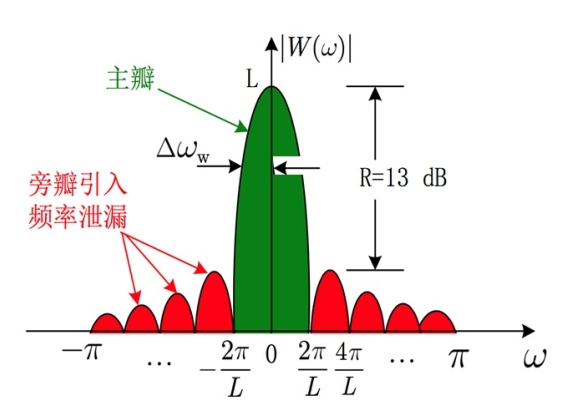
\includegraphics[width=0.6\textwidth]{chap3/img/DTFT_window.png}
        \caption{窗函数的频谱}
        \label{fig:DTFT_window.png}
    \end{figure}
    为方便起见,我们定义它的\bd{主瓣宽度}为
    \begin{align*}
        \Delta\omega_W = \frac{2\pi}{L}.
    \end{align*}
\end{example}

\subsubsection{频谱分辨率}

\begin{example}
    给定信号
    \begin{align*}
        x(n) = A_1\mathe^{\mathi\omega_1 n} + A_2\mathe^{\mathi\omega_2 n},
    \end{align*}
    其中 $n \in \set{Z}, 0 < \omega_1 < \omega_2 < \pi$,
    在一个奈奎斯特区间内,它的 DTFT 为
    \begin{align*}
        X(\omega) = 2\pi(A_1\delta(\omega - \omega_1) + A_2\delta(\omega - \omega_2)).
    \end{align*}
    画出它的频谱如 \ref{fig:DTFT_two_freqs.png} 所示。
    \begin{figure}[H]
        \centering
        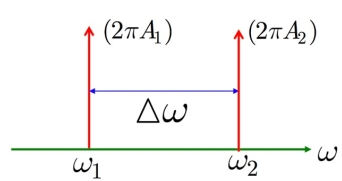
\includegraphics[width=0.3\textwidth]{chap3/img/DTFT_two_freqs.png}
        \caption{两个频率的信号的频谱}
        \label{fig:DTFT_two_freqs.png}
    \end{figure}
    可以看出,这两个频率的间隔为 $\Delta\omega = \omega_2 - \omega_1$。
\end{example}

\begin{example}
    给定信号
    \begin{align*}
        x_L(n) = A_1\mathe^{\mathi\omega_1 n} + A_2\mathe^{\mathi\omega_2 n},
    \end{align*}
    其中 $n \in [0, L-1], 0 < \omega_1 < \omega_2 < \pi$,
    在一个奈奎斯特区间内,它的 DTFT 为
    \begin{align*}
        X_L(\omega) & = \frac{1}{2\pi}X(\omega) \otimes W(\omega) \\
        & = A_1W(\omega - \omega_1) + A_2W(\omega - \omega_2).
    \end{align*}
    画出它的频谱如 \ref{fig:DTFT_two_freqs_window.png} 所示。
    \begin{figure}[H]
        \centering
        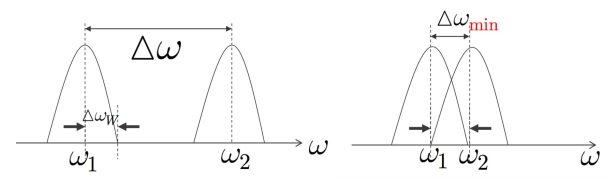
\includegraphics[width=0.6\textwidth]{chap3/img/DTFT_two_freqs_window.png}
        \caption{两个频率的信号的频谱}
        \label{fig:DTFT_two_freqs_window.png}
    \end{figure}
    可以看出,这两个频率的间隔为 $\Delta\omega = \omega_2 - \omega_1$。
\end{example}

\begin{definition}[频谱分辨率]
    那么当 $\Delta\omega$ 很小时,我们如何判断两个频率之间的距离呢?
    或者换而言之,要求分辨出这两个频率,$\Delta\omega$ 至少要多大呢?
    这就引出了\bd{频谱分辨率}的概念。

    当 $\Delta\omega$ 不小于窗函数的主瓣宽度 $\Delta\omega_W = 2\pi/L$ 时,
    我们认为可以分辨出两个频率。也就是说,定义 DTFT 的\bd{频谱分辨率}为
    \begin{align*}
        \Delta\omega_{\min} = \Delta\omega_W = \frac{2\pi}{L},
    \end{align*}
    其中 $L$ 是窗函数的宽度(即序列的长度)。
\end{definition}

\begin{remark}
    序列加窗后会对频谱产生两种影响:
    \begin{enumerate}
        \item 序列频谱中可分辨的最小频率间隔由数据长度决定,
            即窗函数的时间长度。这个现象被称为\bd{不确定原理}。
        \item 序列频谱中出现了高频分量。它们是由于矩形窗
            两个边缘处的突变所造成的。这个现象被称为\bd{频率泄漏}。
            好像是这些原来谱中没有的高频成分是从``内部''(信号原谱分布区间)中
            ``泄漏''出来的一样。显然,这些泄漏量与窗函数的旁瓣有关系,如
            图 \ref{fig:DTFT_leakage.png} 所示。
            \begin{figure}[H]
                \centering
                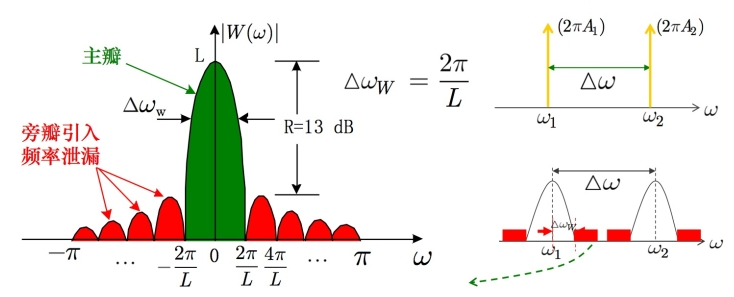
\includegraphics[width=0.6\textwidth]{chap3/img/DTFT_leakage.png}
                \caption{频率泄漏}
                \label{fig:DTFT_leakage.png}
            \end{figure}
    \end{enumerate}
\end{remark}

% \subsection{习题课 2}

\begin{exercise}
    设序列 $x(n) = [2, 3, 6, 1, 0, 1]$,$x(n)$ 的 DTFT 为 $X(\omega)$,
    求 $\int_{-\pi}^{\pi}\|X(\omega)\|^2\D{\omega}$。
\end{exercise}

\begin{solution}
    由帕斯瓦尔定理,有
    \begin{align*}
        \int_{-\pi}^{\pi}\|X(\omega)\|^2\D{\omega} & = 2\pi\sum_{n = 0}^{n = 5}\|x(n)\|^2 \\
        & = 2\pi \times (2^2 + 3^2 + 6^2 + 1^2 + 0^2 + 1^2) \\
        & = 102\pi.
    \end{align*}
\end{solution}

\begin{exercise}
    已知序列 $x(n) = \alpha^n u(-n-1)\cos(\omega_0 n)$,
    其中 $|\alpha| > 1$。
    \begin{enumerate}[label=(\arabic*)]
        \item 求 $x(n)$ 的 DTFT $X(\omega)$。
        \item 利用 DTFT 的帕斯瓦尔定理,计算
            \begin{align*}
                \int_{-\pi}^{\pi}\frac{1}{5 + 4\cos \omega}\D{\omega}.
            \end{align*}
    \end{enumerate}
\end{exercise}

\begin{solution}
    \begin{enumerate}[label=(\arabic*)]
        \item 由题知 $x(n) = \alpha^nu(-n-1) \cdot \frac{1}{2}\left(\mathe^{\mathi\omega_0 n} + \mathe^{-\mathi \omega_0 n}\right)$。
            而
            \begin{align*}
                \DTFT{\alpha^nu(-n-1)} & = \sum_{n = -\infty}^{+\infty}\alpha^nu(-n-1)\mathe^{-\mathi n\omega} \\
                & = \sum_{n = -\infty}^{-1}\left(\alpha\mathe^{-\mathi\omega}\right)^n \\
                & = \sum_{m = 1}^{+\infty}\left(\frac{1}{\alpha\mathe^{-\mathi\omega}}\right)^m \\
                & = \frac{1}{\alpha \mathe^{-\mathi\omega} - 1},
            \end{align*}
            且
            \begin{align*}
                \DTFT{\cos(\omega_0 n)} & = \DTFT{\frac{\mathe^{\mathi\omega_0 n} + \mathe^{-\mathi\omega_0 n}}{2}} \\
                & = \pi(\delta(\omega - \omega_0) + \delta(\omega + \omega_0)),
            \end{align*}
            因此
            \begin{align*}
                X(\omega) & = \frac{1}{2\pi}\DTFT{\alpha^nu(-n-1)} \otimes \DTFT{\cos(\omega_0 n)} \\
                & = \frac{1}{2}\frac{1}{\alpha \mathe^{-\mathi\omega} - 1} \otimes (\delta(\omega - \omega_0) + \delta(\omega + \omega_0)) \\
                & = \frac{1}{2}\left(\frac{1}{\alpha \mathe^{-\mathi(\omega - \omega_0)} - 1} + \frac{1}{\alpha \mathe^{-\mathi(\omega + \omega_0)} - 1}\right).
            \end{align*}
        \item 当 $\omega_0 = 0$ 时,$X(\omega) = 1/(\alpha\mathe^{-\mathi\omega} - 1)$。
            \begin{align*}
                \|X(\omega)\|^2 & = X(\omega)\cdot X^*(\omega) \\
                & = \frac{1}{\alpha\mathe^{-\mathi\omega} - 1} \cdot \frac{1}{\alpha\mathe^{\mathi\omega} - 1} \\
                & = \frac{1}{\alpha^2 + 1 - 2\alpha\cos\omega}.
            \end{align*}
            当 $\alpha = -2$ 时,
            \begin{align*}
                \|X(\omega)\|^2 = \frac{1}{5 + 4\cos\omega}.
            \end{align*}
            此时 $x(n) = (-2)^nu(-n-1)$。因此,由帕斯瓦尔定理,得
            \begin{align*}
                \int_{-\pi}^{\pi}\frac{1}{5 + 4\cos\omega} & = \int_{-\infty}^{+\infty}\|X(\omega)\|^2\D{\omega} \\
                & = 2\pi\sum_{n = -\infty}^{+\infty}|x(n)|^2 \\
                & = 2\pi\sum_{n = -\infty}^{-1}4^n \\
                & = \frac{2\pi}{3}.
            \end{align*}
    \end{enumerate}
\end{solution}

\begin{exercise}
    设序列 $x(n)$ 的 DTFT 为 $X(\omega)$,试用 $X(\omega)$ 表示
    序列 $y(n) = x(2n + 1)$ 的 DTFT $Y(\omega)$。
\end{exercise}

\begin{solution}
    由题知,
    \begin{align*}
        Y(\omega) & = \DTFT{y(n)} \\
        & = \sum_{n = -\infty}^{+\infty}y(n)\mathe^{-\mathi n\omega} \\
        & = \sum_{n = -\infty}^{+\infty}x(2n + 1)\mathe^{-\mathi n\omega} \\
        & = \sum_{k = -\infty}^{+\infty}x(k)\mathe^{-\mathi (k-1)\omega / 2} \cdot \frac{1 - (-1)^k}{2} \\
        & = \frac{1}{2}\sum_{k = -\infty}^{+\infty}x(k)\mathe^{-\mathi (k-1)\omega / 2}
            - \frac{1}{2}\sum_{k = -\infty}^{+\infty}x(k)\mathe^{\mathi k\pi -\mathi (k-1)\omega / 2} \\
        & = \frac{\mathe^{\mathi\omega/2}}{2}\sum_{k = -\infty}^{+\infty}x(k)\mathe^{-\mathi k \omega / 2}
            - \frac{\mathe^{\mathi\omega/2}}{2}\sum_{k = -\infty}^{+\infty}x(k)\mathe^{-\mathi k (\omega / 2 - \pi)} \\
        & = \frac{\mathe^{\mathi\omega/2}}{2}X\left(\frac{\omega}{2}\right)
            - \frac{\mathe^{\mathi\omega/2}}{2}X\left(\frac{\omega}{2} - \pi\right).
    \end{align*}
\end{solution}

\begin{note}
    以下是常见错误解法:
    \begin{enumerate}
        \item 错误解法 1:
            \begin{align*}
                \DTFT{x(2n + 1)} = \DTFT{x_{1/2}\left(n + \frac{1}{2}\right)} = \mathe^{\mathi\omega/2}X\left(\frac{\omega}{2}\right).
            \end{align*} 
            这是因为只有\bd{当 $a$ 为非零整数时},才能使用时域扩展公式
            \begin{align*}
                x_{(a)}(n) = \begin{cases}
                    x\left(\frac{n}{a}\right), & \frac{n}{a} \in \set{Z}, \\
                    0, & \text{otherwise}.
                \end{cases}
            \end{align*}
        \item 错误解法 2:
            \begin{align*}
                \DTFT{x(2n + 1)} = \sum_{n = -\infty}^{+\infty}x(2n + 1)\mathe^{-\mathi n\omega}
                    = \sum_{m = -\infty}^{+\infty}x(m)\mathe^{-\mathi (m - 1)\omega / 2}
                    = \mathe^{\mathi\omega/2}X\left(\frac{\omega}{2}\right).
            \end{align*}
            这是因为只有\bd{当 $m$ 为奇数时}才应当被计入和式,第二个等号不成立。
        \item 错误解法 3:
            \begin{align*}
                \DTFT{x(2n + 1)} = \mathe^{-\mathi\omega(-1)}\DTFT{x(2n)}
                    = \frac{1}{2}\mathe^{\mathi\omega}\left[X\left(\frac{\omega}{2}\right)
                        + X\left(\frac{\omega}{2} - \pi\right)\right].
            \end{align*}
            这是因为时域平移公式只适用于 \bd{$n_0$ 为整数}的情况:
            \begin{align*}
                \DTFT{x(n - n_0)} = \mathe^{-\mathi n_0\omega}X(\omega),
            \end{align*}
            其中 $n_0 \in \set{Z}$。
    \end{enumerate}
\end{note}

\begin{exercise}
    已知序列 $x(n)$ 和 $y(n)$ 的 DTFT 分别为 $X(\omega)$ 和 $Y(\omega)$。
    \begin{enumerate}[label=(\arabic*)]
        \item 试用 $X(\omega)$ 表示序列 $x_1(n) = x(4n)$ 的 DTFT $X_1(\omega)$。
        \item 对周期函数 $X(\omega)$ 和 $Y(\omega)$,定义相关系数
            \begin{align*}
                R_{XY}(\omega) = \int_{-\pi}^{\pi}X(\omega' + \omega)Y^*(\omega')\D{\omega'}
                    = \int_{-\pi}^{\pi}X(\omega')Y^*(\omega' - \omega)\D{\omega'}.
            \end{align*}
            记 $R_{XY}(\omega)$ 的 IDTFT 为 $r_{xy}(n)$,
            试用 $x(n)$ 和 $y(n)$ 表示 $r_{xy}(n)$。
    \end{enumerate}
\end{exercise}

\begin{solution}
    \begin{enumerate}[label=(\arabic*)]
        \item 令 $h(n) = x(2n)$,则
            \begin{align*}
                H(\omega) & = \DTFT{h(n)} \\
                & = \DTFT{x(2n)} \\
                & = \frac{1}{2}\left(X\left(\frac{\omega}{2}\right) + X\left(\frac{\omega}{2} - \pi\right)\right),
            \end{align*}
            故
            \begin{align*}
                H\left(\frac{\omega}{2}\right) = \frac{1}{2}\left(X\left(\frac{\omega}{4}\right) + X\left(\frac{\omega}{4} - \pi\right)\right),
                H\left(\frac{\omega}{2} - \pi\right) = \frac{1}{2}\left(X\left(\frac{\omega}{4} - \frac{\pi}{2}\right) + X\left(\frac{\omega}{4} - \frac{3}{2}\pi\right)\right).
            \end{align*}
            因此
            \begin{align*}
                X_1(\omega) & = \frac{1}{2}\left(H\left(\frac{\omega}{2}\right) + H\left(\frac{\omega}{2} - \pi\right)\right) \\
                & = \frac{1}{4}\left(X\left(\frac{\omega}{4}\right) + X\left(\frac{\omega}{4} - \pi\right) + X\left(\frac{\omega}{4} - \frac{\pi}{2}\right) + X\left(\frac{\omega}{4} - \frac{3}{2}\pi\right)\right).
            \end{align*}
        \item 由于
            \begin{align*}
                R_{XY}(\omega) & = \int_{-\pi}^{\pi}X(\omega' + \omega)Y^*(\omega')\D{\omega'} \\
                & = X(\omega) \otimes Y^*(-\omega),
            \end{align*}
            故
            \begin{align*}
                r_{xy}(n) & = \IDTFT{X(\omega) \otimes Y^*(-\omega)} \\
                & = 2\pi \cdot \IDTFT{X(\omega)} \cdot \IDTFT{Y^*(-\omega)} \\
                & = 2\pi x(n)y^*(n).
            \end{align*}
    \end{enumerate}
\end{solution}

\begin{remark}
    在此题中,构造
    \begin{align*}
        C(m) = \frac{1}{4}\left(1 + \mathe^{\frac{1}{4}\mathi \cdot 2m\pi}
            + \mathe^{\frac{2}{4}\mathi \cdot 2m\pi}
            + \mathe^{\frac{3}{4}\mathi \cdot 2m\pi}\right)
    \end{align*}
    可以直接求 $\DTFT{x(4n)}$。其中 $C(m)$ 也满足
    \begin{align*}
        C(m) = \begin{cases}
            1, & m \equiv 0 \pmod{4}, \\
            0, & \text{otherwise}.
        \end{cases}
    \end{align*}
\end{remark}

\begin{note}
    事实上,对于任意的 $n \in \set{Z}$,可以构造
    \begin{align*}
        C(m) = \begin{cases}
            1, & m \equiv 0 \pmod{n}, \\
            0, & \text{otherwise}.
        \end{cases}
    \end{align*}
    从而可以直接求 $\DTFT{x(nm)}$。构造
    \begin{align*}
        C(m) & = \frac{1}{n}\sum_{k = 0}^{n-1}\mathe^{2m\pi\mathi \cdot k/n} \\
        & = \frac{1}{n}\sum_{k = 0}^{n - 1}\left(\mathe^{2\pi\mathi \cdot m/n}\right)^k,
    \end{align*}
    \begin{itemize}
        \item 当 $n \nmid m$ 时,$\mathe^{2\pi\mathi \cdot m/n} \neq 1$,
            \bd{这是一个等比数列},因此
            \begin{align*}
                C(m) & = \frac{1}{n}\cdot 1 \times \frac{1 - \mathe^{2\pi\mathi \cdot m}}{1 - \mathe^{2\pi\mathi \cdot m/n}} \\
                & = 0.
            \end{align*}
        \item 当 $n \mid m$ 时,$\mathe^{2\pi\mathi \cdot m/n} = 1$,
            \bd{这是一个常数列},故 $C(m) = \frac{1}{n} \times n = 1$。
    \end{itemize}
    这样构造出的 $C(m)$ 是满足要求的。
\end{note}

\begin{exercise}
    已知序列 $h(n) = (1/2)^nu(n)$,其中 $u(n) = \begin{cases}
        1, & n \ge 0, \\
        0, & n < 0.
    \end{cases}$
    \begin{enumerate}[label=(\arabic*)]
        \item $x(n) = \cos(\omega_0 n)$,求 $\DTFT{h(n)x(n)}$。
        \item 求 $y(n) = h(n) * (-1)^n$。
        \item 利用 DTFT 的帕斯瓦尔定理,计算
            \begin{align*}
                \int_{-\pi}^{\pi}\frac{1}{5 - 4\cos\omega}\D{\omega}.
            \end{align*}
    \end{enumerate}
\end{exercise}

\begin{solution}
    \begin{enumerate}[label=(\arabic*)]
        \item 不妨设 $h(n)$ 和 $x(n)$ 的 DTFT 分别为 $H(\omega)$ 和 $X(\omega)$。
            则
            \begin{align*}
                H(\omega) & = \sum_{n = -\infty}^{+\infty}h(n)\mathe^{-\mathi n\omega} \\
                & = \sum_{n = 0}^{+\infty}\left(\frac{1}{2}\right)^n\mathe^{-\mathi n\omega} \\
                & = \frac{1}{1 - \frac{1}{2}\mathe^{-\mathi\omega}},
            \end{align*}
            且
            \begin{align*}
                X(\omega) & = \DTFT{\frac{\mathe^{\mathi\omega n} + \mathe^{-\mathi\omega n}}{2}} \\
                & = \pi(\delta(\omega - \omega_0) + \delta(\omega + \omega_0)).
            \end{align*}
            由 DTFT 的性质,可知
            \begin{align*}
                \DTFT{h(n)x(n)} & = \frac{1}{2\pi}H(\omega) \oplus X(\omega) \\
                & = \frac{1}{2\pi}\cdot\left(\frac{1}{1 - \frac{1}{2}\mathe^{-\mathi\omega}} \oplus (\delta(\omega - \omega_0) + \delta(\omega + \omega_0))\right) \\
                & = \frac{1}{2 - \mathe^{-\mathi(\omega - \omega_0)}} + \frac{1}{2 - \mathe^{-\mathi(\omega + \omega_0)}}.
            \end{align*}
        \item 由卷积的定义,知
            \begin{align*}
                y(n) & = \sum_{m = -\infty}^{+\infty}h(m)(-1)^{n-m} \\
                & = (-1)^n\sum_{m = 0}^{+\infty}\left(-\frac{1}{2}\right)^m \\
                & = (-1)^n\cdot \frac{1}{1 + \frac{1}{2}} \\
                & = \frac{2}{3}(-1)^n.
            \end{align*}
        \item 注意到
            \begin{align*}
                \|H(\omega)\|^2 & = H(\omega) \cdot H^*(\omega) \\
                & = \frac{1}{1 - \frac{1}{2}\mathe^{-\mathi\omega}} \cdot \frac{1}{1 - \frac{1}{2}\mathe^{\mathi\omega}} \\
                & = \frac{4}{5 - 4\cos\omega},
            \end{align*}
            因此,
            \begin{align*}
                \int_{-\pi}^{\pi}\frac{1}{5 - 4\cos\omega}\D{\omega} & = \frac{1}{4}\int_{-\pi}^{\pi}\|H(\omega)\|^2\D{\omega} \\
                & = \frac{1}{4}\times 2\pi\sum_{n = -\infty}^{+\infty}|h(n)|^2 \\
                & = \frac{\pi}{2}\sum_{n = 0}^{+\infty}\left(\frac{1}{4}\right)^{n} \\
                & = \frac{2\pi}{3}.
            \end{align*}
    \end{enumerate}
\end{solution}

% \subsection{离散傅里叶变换}

离散时间信号的傅里叶频谱是连续的,而计算机只能处理离散的数据,
因此需要将连续的频谱离散化,这就是离散傅里叶变换。

\subsubsection{离散傅里叶变换的定义}

\begin{definition}
    由长度为 $L$ 的序列 $x(n), n = 0, 1, \cdots, L - 1$,
    求其 DTFT 谱上 $[0, 2\pi]$ 区间上均匀分布的 $N$ 个谱值
    \begin{align*}
        \omega_k = \frac{2\pi k}{N}, \quad k = 0, 1, \cdots, N - 1,
    \end{align*}
    的过程称为\bd{离散傅里叶变换}(DFT),记为
    \begin{align*}
        X'(\omega_k) = \sum_{n = 0}^{L - 1}x(n)\mathe^{-\mathi\omega_k n}.
    \end{align*}
    将其写为 $k$ 的函数形式,即
    \begin{align*}
        X(k) = \sum_{n = 0}^{L - 1}x(n)\mathe^{-2\pi\mathi k n/N}.
    \end{align*}
    记 $W_N = \mathe^{-2\pi\mathi/N}$,则
    \begin{align*}
        X(k) = \sum_{n = 0}^{L - 1}x(n)W_N^{kn},
    \end{align*}
    其中 $k = 0, 1, \cdots, N - 1$。
\end{definition}

\begin{exercise}
    利用 DFT 的公式计算
    \begin{align*}
        x(n) = \sin\left(\frac{2\pi}{N}mn\right)
    \end{align*}
    的 $N$ 点 DFT,其中 $0 \le n \le N - 1, 0 < m < N$ 且 $m \in \set{Z}$。
\end{exercise}

\begin{solution}
    由于 $\sin\theta = (\mathe^{\mathi\theta} - \mathe^{-\mathi\theta})/(2\mathi)$,因此
    \begin{align*}
        x(n) & = \sin\left(\frac{2\pi}{N}mn\right) \\
        & = \frac{\mathe^{2\pi\mathi mn/N} - \mathe^{-2\pi\mathi mn/N}}{2\mathi} \\
        & = \frac{\mathi}{2} \left(W_N^{mn} - W_N^{-mn}\right).
    \end{align*}
    由 DFT 的定义可知
    \begin{align*}
        X(k) & = \sum_{n = 0}^{N - 1} x(n)W_N^{kn} \\
        & = \sum_{n = 0}^{N - 1} \sin\left(\frac{2\pi}{N}mn\right)W_N^{kn} \\
        & = \frac{\mathi}{2}\sum_{n = 0}^{N - 1}\left(W_N^{mn} - W_N^{-mn}\right)W_N^{kn} \\
        & = \frac{\mathi}{2}\sum_{n = 0}^{N - 1}W_N^{(k + m)n} - \frac{\mathi}{2}\sum_{n = 0}^{N - 1}W_N^{(k - m)n}.
    \end{align*}
    当 $k + m = N$ 时,$\frac{\mathi}{2}\sum_{n = 0}^{N - 1}W_N^{(k + m)n} = \mathi N / 2$。
    当 $k + m \neq N$ 时,$\frac{\mathi}{2}\sum_{n = 0}^{N - 1}W_N^{(k + m)n}$ 为等比数列求和,故
    \begin{align*}
        \frac{\mathi}{2}\sum_{n = 0}^{N - 1}W_N^{(k + m)n} & = \frac{\mathi}{2}\frac{1 - \left(W_N^{k + mN}\right)^N}{1 - W_N^{k + m}} \\
        & = 0.
    \end{align*}
    当 $k = m$ 时,$\frac{\mathi}{2}\sum_{n = 0}^{N - 1}W_N^{(k - m)n} = \mathi N / 2$。
    当 $k \ne m$ 时,$\frac{\mathi}{2}\sum_{n = 0}^{N - 1}W_N^{(k - m)n}$ 为等比数列求和,故
    \begin{align*}
        \frac{\mathi}{2}\sum_{n = 0}^{N - 1}W_N^{(k - m)n} & = \frac{\mathi}{2} \cdot \frac{1 - \left(W_N^{k - m}\right)^N}{1 - W_N^{k - m}} \\
        & = 0.
    \end{align*}
    综上所述,
    \begin{align*}
        X(k) = \frac{\mathi N}{2}(\delta(k + m - N) - \delta(k - m)).
    \end{align*}
\end{solution}

\subsubsection{DFT 的矩阵表示}

\begin{definition}[DFT 的矩阵表示]
    如果将 $x(n)$ 看作是一个列向量 $\vct{x}$,将 $X(k)$ 看作是一个列向量 $\vct{X}$,
    则 DFT 可以表示为
    \begin{align*}
        \vct{X} = \begin{bmatrix}
            X_0 \\ X_1 \\ \vdots \\ X_{N - 1}
        \end{bmatrix}
        = A \begin{bmatrix}
            x_0 \\ x_1 \\ \vdots \\ x_{L - 1}
        \end{bmatrix} = A\vct{x},
    \end{align*}
    其中 $A$ 是 DFT 的矩阵表示,即
    \begin{align*}
        A_{kn} = W_N^{kn} = \mathe^{-2\pi\mathi kn/N}.
    \end{align*}
    这是因为由 DFT 的定义,有
    \begin{align*}
        X_k = \sum_{n = 0}^{L - 1}W_N^{kn}x_n,
    \end{align*}
\end{definition}

\subsubsection{$N$ 与 $L$ 的关系}

从理论上讲,DFT 中的 $N$ 与 $L$ 之间是相互独立的。$L$ 是数据记录中
时域样本的数目,它可能是无限的;而 $N$ 则是对 DTFT 进行采样时的频率点的数目。
通常,在讨论和使用 DFT(特别是编程实现)时常常取 $N = L$。
既然 $L$ 与 $N$ 没有什么必然的联系,那么,为什么要设它们相等?
这是出于什么考虑呢?

\begin{example}[$N > L$ 的情况]
    $N > L$ 说明频域的采样点个数 $N$ 比序列的长度 $L$ 多,
    此时只需要在序列尾部补\bd{任意数目}的 $0$ 即可。新序列的 DFT 与原序列的 DFT 结果
    相同。
\end{example}

\begin{theorem}
    设长度为 $L$ 的序列 $x(n)$ 的 DFT 为 $X(k)$,则将其补 $N - L$ 个 $0$,
    设得到的新序列为 $x_D(n)$,其 DFT 为 $X_D(k)$。用向量表示为
    \begin{align*}
        \vct{x} = \begin{bmatrix}
            x_0 \\ x_1 \\ \vdots \\ x_{L - 1}
        \end{bmatrix}, \quad
        \vct{x}_D = \begin{bmatrix}
            x_0 \\ x_1 \\ \vdots \\ x_{L - 1} \\ 0 \\ \vdots \\ 0
        \end{bmatrix}.
    \end{align*}
    此时,有
    \begin{align*}
        X_D(k) = X(k).
    \end{align*}
\end{theorem}
    
\begin{proof}
    由 DFT 的定义可知
    \begin{align*}
        X_D(k) & = \sum_{n = 0}^{N - 1}x_D(n)W_N^{kn} \\
        & = \sum_{n = 0}^{L - 1}x(n)W_N^{kn} \\
        & = X(k).
    \end{align*}
\end{proof}

\begin{definition}[回绕序列]
    设有序列 $x(n)$ 的长度为 $L$,则定义其关于 $N(N < L)$ 的\bd{回绕序列}为
    \begin{align*}
        \rev{x}(n) = \sum_{m = 0}^{+\infty}x(mN + n),
    \end{align*}
    其中 $n = 0, 1, \cdots, N - 1$。
    这类似于将长度为 $L$ 的序列切成每块长度为 $N$ 的子序列,然后将这些子序列按位相加,
    如果一块子序列的长度不足 $N$,则在末尾补 $0$。如图 \ref{fig:wrapped_sequence} 所示。
    \begin{figure}[H]
        \centering
        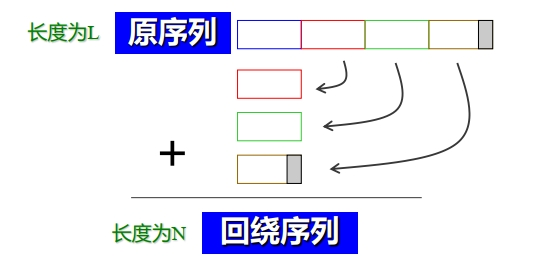
\includegraphics[width = 0.6\textwidth]{chap3/img/wrapped_sequence.png}
        \caption{回绕序列的示意图}
        \label{fig:wrapped_sequence}
    \end{figure}
\end{definition}

\begin{example}[$N < L$ 的情况]
    当 $N < L$ 时,频域的采样点个数 $N$ 少于序列的长度 $L$,此时可以将序列转为
    其回绕序列,再进行 DFT。回绕序列的 DFT 与原序列的 DFT 结果相同。
\end{example}

\begin{theorem}
    设长度为 $L$ 的序列 $x(n)$ 的 DFT 为 $X(k)$,
    其回绕序列 $\rev{x}(n)$ 的 DFT 为 $\rev{X}(k)$。
    则有
    \begin{align*}
        \rev{X}(k) = X(k).
    \end{align*}
\end{theorem}

\begin{proof}
    (方法一)
    由于 $A_{k, mN + n} = W_N^{(mN + n)k} = W_N^{nk} = A_{k, n}$,
    故
    \begin{align*}
        A = \begin{bmatrix}
            B & B & \cdots
        \end{bmatrix}
    \end{align*}
    其中 $B$ 是 $N \times N$ 的矩阵,$B_{kn} = W_N^{kn}$。则
    \begin{align*}
        \vct{X} = A\vct{x} = \begin{bmatrix}
            B & B & \cdots
        \end{bmatrix} \vct{x}
        = B\begin{bmatrix}
            I_N & I_N & \cdots
        \end{bmatrix}\vct{x}
        = B\vct{\rev{x}} = \vct{\rev{X}}.
    \end{align*}
\end{proof}

\begin{proof}
    (方法二)
    由 DFT 的定义可知 $X(k) = \sum_{n = 0}^{L - 1}x(n)W_N^{nk}$。不妨设 $N \mid L$,
    因为如果 $N \nmid L$,则可以将 $x(n)$ 补 $N - L$ 个 $0$,使得 $N' \mid L$。
    由于 $N \mid L$,故 $L = Nq$,其中 $q$ 为正整数。则
    \begin{align*}
        \rev{X}(k) & = \sum_{n = 0}^{N - 1}\rev{x}(n)W_N^{nk} \\
        & = \sum_{n = 0}^{N - 1}\sum_{m = 0}^{q - 1}x(mN + n)W_N^{nk}.
    \end{align*}
    由于 $W_N^{(mN + n)k} = \mathe^{-2\pi\mathi k(mN + n)/N}
        = \mathe^{-2\pi\mathi kn} = W_N^{kn}$,
    故
    \begin{align*}
        \rev{X}(k) & = \sum_{n = 0}^{N - 1}\sum_{m = 0}^{q - 1}x(mN + n)W_N^{nk} \\
        & = \sum_{m = 0}^{q - 1}\sum_{n = 0}^{N - 1}x(mN + n)W_N^{(mN + n)k}.
    \end{align*}
    注意到此时 $mN + n$ 遍历了 $0, 1, \cdots, L - 1$,故
    \begin{align*}
        \rev{X}(k) & = \sum_{m = 0}^{q - 1}\sum_{n = 0}^{L - 1}x(n)W_N^{nk} \\
        & = \sum_{n = 0}^{L - 1}x(n)W_N^{nk} \\
        & = X(k).
    \end{align*}
    命题得证。
\end{proof}

\begin{remark}
    多个完全不同的序列,只要它们的回绕序列相等,它们的 DFT 也就相等。
    从 IDFT 只能得到唯一的一个序列,实际上对应所有序列的回绕序列。
    如图 \ref{fig:wrapped_sequence_relation} 所示。
    \begin{figure}[H]
        \centering
        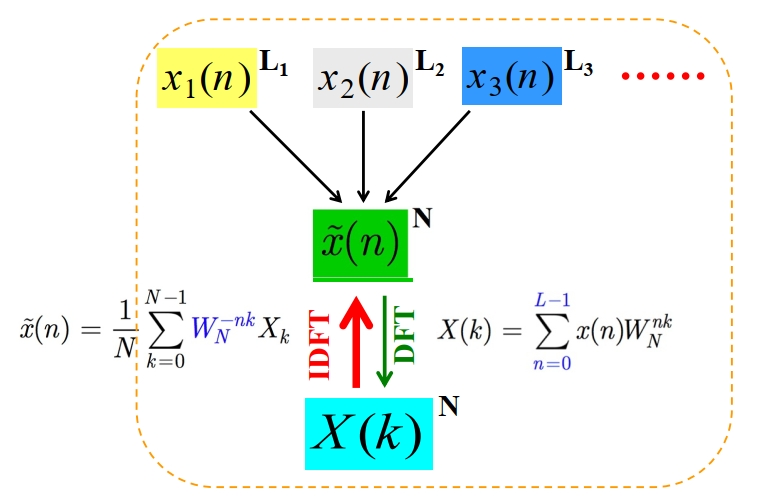
\includegraphics[width = 0.6\textwidth]{chap3/img/wrapped_sequence_relation.png}
        \caption{回绕序列的 DFT 与 IDFT 的关系}
        \label{fig:wrapped_sequence_relation}
    \end{figure}
\end{remark}

\begin{corollary}[$N$ 与 $L$ 的关系]
    DFT、IDFT 中序列的长度 $L$ 与频域采样点个数 $N$ 之间的关系如下:
    \begin{enumerate}[label=(\arabic*)]
        \item $L$ 是待处理的数据长度,不可更改;而 $N$ 则只是数字处理设备中的算法
            参数,由设计人员在使用时设定。
        \item 若 $N > L$,则在数值计算中相当于在序列后面补 $0$,使得 $L = N$。
            虽然这不影响 DFT 结果的正确性,但因补充的 $0$ 使得计算量增大,
            浪费了计算资源。
        \item 若 $N < L$,则可以将序列转为其回绕序列,再进行 DFT。回绕序列的 DFT
            与原序列的 DFT 结果相同。但是回绕序列与原序列的关系是多对一的,
            因此 IDFT 只能得到唯一的一个序列,实际上对应所有序列的回绕序列。
        \item 只有在 $N \ge L$ 时,才能保证 IDFT 的唯一性。
    \end{enumerate}
    结论是,\bd{为了方便计算,通常取 $N = L$}。
\end{corollary}

\subsubsection{离散傅里叶变换的性质}

\begin{property}[DFT 的离散性、周期性]
    设 $x(n)$ 的 DFT 为 $X(k)$,则 $X(k)$ 只能在 $k = 0, 1, \cdots, N - 1$ 处
    取值,且
    \begin{align*}
        X(k) = X(k + N), \quad k = 0, 1, \cdots, N - 1.
    \end{align*}
\end{property}

\begin{property}[DFT 的共轭对称性]
    设 $x(n)$ 为实序列,则
    \begin{align*}
        X^*(N - k) = X(k), \quad k = 1, \cdots, N - 1.
    \end{align*}
\end{property}

\begin{note}
    这里 $k$ 的取值范围是 $[1, N-1]$,这是因为定义域要求
    \begin{align*}
        \begin{cases}
            0 \le N - k \le N - 1, \\
            0 \le k \le N - 1.
        \end{cases}
    \end{align*}
    解得 $1 \le k \le N - 1$。
\end{note}

\begin{proof}
    由于 $W_N = \mathe^{-2\pi\mathi/N}$,因此
    \begin{align*}
        \left(W_N^{(N - k)n}\right)^* & = \left(\mathe^{-2\pi\mathi n(N-k)/N}\right)^* \\
        & = \mathe^{-2\pi\mathi n(k-N)/N} \\
        & = \mathe^{-2\pi\mathi kn/N} \cdot \mathe^{2\pi\mathi n} \\
        & = \left(\mathe^{-2\pi\mathi/N}\right)^{kn} \\
        & = W_N^{kn}.
    \end{align*}
    由于 $x(n)$ 为实序列,故 $x(n) = x^*(n)$,所以由 DFT 的定义可知
    \begin{align*}
        X^*(N - k) & = \left(\sum_{n = 0}^{N - 1} x(n)W_N^{(N - k)n}\right)^* \\
        & = \sum_{n = 0}^{N - 1} x^*(n)\left(W_N^{(N - k)n}\right)^* \\
        & = \sum_{n = 0}^{N - 1} x(n)W_N^{kn} \\
        & = X(k).
    \end{align*}
    命题得证。
\end{proof}

\begin{property}[DFT 是线性运算]
    设 $x_1(n)$ 和 $x_2(n)$ 的 DFT 分别为 $X_1(k)$ 和 $X_2(k)$,则
    \begin{align*}
        \DFT{a_1x_1(n) + a_2x_2(n)} = a_1X_1(k) + a_2X_2(k).
    \end{align*}
\end{property}

\begin{property}[DFT 的帕斯瓦尔定理]
    设长度为 $L$ 的序列 $x(n)$ 的 DFT 为长度为 $N$ 的频谱 $X(k)$,
    当 $L = N$ 时,有
    \begin{align*}
        \sum_{n = 0}^{N - 1}\|x(n)\|^2 = \frac{1}{N}\sum_{k = 0}^{N - 1}\|X(k)\|^2.
    \end{align*}
\end{property}

\begin{property}[DFT 的奇偶性、虚实性]
    对于奇对称序列、偶对称序列、实序列、虚序列,其 DFT 的性质如下:
    \begin{enumerate}
        \item 奇对称和偶对称序列:
            \begin{itemize}
                \item 奇对称序列的 DFT 是奇对称序列。
                \item 偶对称序列的 DFT 是偶对称序列。
            \end{itemize}
        \item 实序列:
            \begin{itemize}
                \item 实偶序列的 DFT 是实偶序列,实奇序列的 DFT 是虚奇序列。
                \item 实序列的 DFT 的实部是偶序列,虚部是奇序列。
                \item 实序列的 DFT 的模长序列是偶序列,相位序列是奇序列。
            \end{itemize}
        \item 虚序列:
            \begin{itemize}
                \item 虚偶序列的 DFT 是虚偶序列,虚奇序列的 DFT 是实奇序列。
                \item 虚序列的 DFT 的实部是奇序列,虚部是偶序列。
                \item 虚序列的 DFT 的模长序列是偶序列,相位序列是奇序列。
            \end{itemize}
    \end{enumerate}
\end{property}

\begin{property}[DFT 的反褶和共轭的性质]
    设信号 $x(n)$ 的 DFT 为 $X(k)$,则进行反褶和共轭操作后的信号的 DFT 对应关系如下:
    \begin{figure}[H]
        \begin{tabular}
            {c||c|c}
            操作 & 时域 & 频域 \\
            \hline
            反褶 & $x(-n)$ & $X(-k)$ \\
            共轭 & $x^*(n)$ & $X^*(-k)$ \\
            反褶且共轭 & $x^*(-n)$ & $X^*(k)$ \\
        \end{tabular}
    \end{figure}
\end{property}

\begin{property}[DFT 的频移特性]
    设长度为 $L$ 的序列 $x(n)$ 的 DFT 为长度为 $N$ 的频谱 $X(k)$,
    当 $L = N$ 时,有
    \begin{align*}
        X(k - k_0) = \DFT{x(n)W_N^{-k_0n}}.
    \end{align*}
\end{property}

\begin{proof}
    由 DFT 的定义可知
    \begin{align*}
        X(k - k_0) & = \sum_{n = 0}^{N - 1}x(n)W_N^{(k - k_0)n} \\
        & = \sum_{n = 0}^{N - 1}\left(x(n)W_N^{-k_0n}\right)W_N^{kn} \\
        & = \DFT{x(n)W_N^{-k_0n}}.
    \end{align*}
    命题得证。
\end{proof}

\begin{property}[DFT 的对称性]
    设长度为 $L$ 的序列 $x(n)$ 的 DFT 为长度为 $N$ 的频谱 $X(k)$,
    当 $L = N$ 时,有
    \begin{align*}
        \DFT{X(n)} = N\rev{x}(-k).
    \end{align*}
\end{property}

\begin{proof}
    由 IDFT 的定义,
    \begin{align*}
        \rev{x}(n) = \frac{1}{N}\sum_{k = 0}^{N - 1}X(k)W_N^{-kn}.
    \end{align*}
    因此
    \begin{align*}
        N\rev{x}(-n) = \sum_{k = 0}^{N - 1}X(k)W_N^{kn}.
    \end{align*}
    将自变量改写为 $n$,即可得到
    \begin{align*}
        N\rev{x}(-k) = \sum_{n = 0}^{N - 1}X(n)W_N^{kn} = \DFT{X(n)}.
    \end{align*}
    命题得证。
\end{proof}

\begin{property}[DFT 的时移特性]
    设长度为 $L$ 的序列 $x(n)$ 的 DFT 为长度为 $N$ 的频谱 $X(k)$,有
    \begin{align*}
        \DFT{x(n - m)} = W_N^{mk}X(k).
    \end{align*}
\end{property}

\begin{proof}
    (方法一)
    DTFT 的时移特性为 $\DTFT{x(n - m)} = \mathe^{-\mathi\omega m}X(\omega)$。
    由于 DFT 可以看做是 DTFT 在离散点上的采样,故
    \begin{align*}
        \DFT{x(n - m)} & = \left.\left(\mathe^{-\mathi\omega m}X(\omega)\right)\right|_{\omega = \omega_k} \\
        & = \mathe^{-\mathi\omega_k m}X(\omega_k) \\
        & = W_N^{mk}X(k).
    \end{align*}
\end{proof}

\begin{proof}
    (方法二)
    最需要处理的情况是当 $n < m$ 时 $x(n - m)$ 应该如何对应到 $X(k)$。
    可以考虑定义回绕序列
    \begin{align*}
        \rev{x}(n - m) = \begin{cases}
            x(n + N - m), & 0 \le n < m, \\
            x(n - m), & m \le n < N.
        \end{cases}
    \end{align*}
    显然它们的 DFT 是相等的,即
    \begin{align*}
        \DFT{x(n - m)} = \DFT{\rev{x}(n - m)}.
    \end{align*}
    由 DFT 的定义可知
    \begin{align*}
        \DFT{x(n - m)} & = \DFT{\rev{x}(n - m)} \\
        & = \sum_{n = 0}^{m - 1}x(n - m + N)W_N^{kn}
            + \sum_{n = m}^{N - 1}x(n - m)W_N^{kn} \\
        & = \left(\sum_{n = 0}^{m - 1}x(n - m + N)W_N^{(n - m + N)k}
            + \sum_{n = m}^{N - 1}x(n - m)W_N^{(n - m)k}\right)W_N^{mk} \\
        & = \left(\sum_{t = N - m}^{N - 1}x(t)W_N^{tk}
            + \sum_{n = 0}^{N - m - 1}x(t)W_N^{tk}\right)W_N^{mk} \\
        & = \left(\sum_{t = 0}^{N - 1}x(t)W_N^{tk}\right)W_N^{mk} \\
        & = X(k)W_N^{mk}. 
    \end{align*}
    命题得证。
\end{proof}

\begin{property}[DFT 的时域卷积特性]
    设序列 $x_1(n)$ 和 $x_2(n)$ 的 DFT 分别为 $X_1(k)$ 和 $X_2(k)$,
    则
    \begin{align*}
        \DFT{x_1(n) * x_2(n)} = X_1(k)X_2(k),
    \end{align*}
    其中 $x_1(n) * x_2(n) = \sum_{m = -\infty}^{+\infty}x_1(m)x_2(n - m)$。
\end{property}

\begin{property}[DFT 的频域卷积特性]
    设序列 $x_1(n)$ 和 $x_2(n)$ 的 DFT 分别为 $X_1(k)$ 和 $X_2(k)$,
    则
    \begin{align*}
        \DFT{x_1(n)x_2(n)} = \frac{1}{N}X_1(k) \otimes X_2(k),
    \end{align*}
\end{property}

\begin{property}[IDFT 的频域卷积特性]
    设长度为 $L$ 的序列 $x(n)$ 和 $y(n)$ 的 DFT 分别为长度为 $N$ 的序列 $X(k)$ 和 $Y(k)$,
    当 $N = L$ 时,有
    \begin{align*}
        \IDFT{X(k)Y(k)} = \rev{x(n) * y(n)}
        = \sum_{m = 0}^{N - 1}x(m)\rev{y}(n - m)
        = \sum_{m = 0}^{N - 1}x(m)y(n - m)_N = x(n) \otimes y(n).
    \end{align*}
\end{property}

\begin{proof}
    由于 $\IDFT{Z(k)} = \rev{z}(n)$,因此
    \begin{align*}
        \IDFT{X(k)Y(k)} = \rev{x(n) * y(n)}.
    \end{align*}
    将 IDFT 的定义代入,即可得到
    \begin{align*}
        \IDFT{X(k)Y(k)} & = \frac{1}{N}\sum_{k = 0}^{N - 1}X(k)Y(k)W_N^{-nk} \\
        & = \frac{1}{N}\sum_{k = 0}^{N - 1}\sum_{m = 0}^{N - 1}x(m)W_N^{mk}Y(k)W_N^{-nk} \\
        & = \sum_{m = 0}^{N - 1}x(m)\left(\frac{1}{N}\sum_{k = 0}^{N - 1}Y(k)W_N^{mk}W_N^{-nk}\right) \\
        & = \sum_{m = 0}^{N - 1}x(m)\IDFT{Y(k)W_N^{mk}} \\
        & = \sum_{m = 0}^{N - 1}x(m)\rev{y}(n - m).
    \end{align*}
    考虑到回绕一个移位序列相当于循环移位,所以 $\rev{y}(n - m) = y(n - m)_N$,故
    \begin{align*}
        \IDFT{X(k)Y(k)} = \sum_{m = 0}^{N - 1}x(m)y(n - m)_N = x(n) \otimes y(n).
    \end{align*}
    命题得证。
\end{proof}

\begin{remark}
    计算的过程为:反褶、循环移位、相乘、相加。

    $\otimes$ 也是一种卷积,为了突出新卷积与旧卷积的不同,
    同时也为了突出它们之间的相同, 称过去传统的卷积为\bd{线卷积},
    而称此新卷积为序列的圆周卷积,简称\bd{圆卷积}。
\end{remark}

\subsubsection{总结:FT、DTFT、DFT 的性质}

\begin{figure}[H]
    \centering
    \begin{tabular}{c||p{3cm}|p{4cm}|p{4cm}}
        \textbf{ } & \textbf{FT} & \textbf{DTFT} & \textbf{DFT} \\
        \hline
        线性性 & 是 & 是 & 是 \\
        \hline
        时域反褶 & 频域反褶 & 频域反褶 & 频域反褶 \\
        \hline
        时域共轭 & 频域共轭+反褶 & 频域共轭+反褶 & 频域共轭+反褶 \\
        \hline
        对称性 & $\mathcal{F}[F(t)] = 2\pi f(-\omega)$
            & $\DTFT{X(n)} = 2\pi x(-\omega)$
            & $\DFT{X(n)} = N \rev{x}(-k)$ \\
        \hline
        时域平移 & $\mathcal{F}[f(t - t_0)] = \mathe^{-\mathi\omega t_0}F(\omega)$
            & $\DTFT{x(n - n_0)} = \mathe^{-\mathi\omega n_0}X(\omega)$
            & $\DFT{x(n - n_0)} = W_N^{kn_0}X(k)$ \\
        \hline
        频域平移 & $\mathcal{F}[\mathe^{\mathi\omega_0 t}f(t)] = F(\omega - \omega_0)$
            & $\DTFT{\mathe^{\mathi\omega_0 n}x(n)} = X(\omega - \omega_0)$
            & $\DFT{x(n)W_N^{-nk_0}} = X(k - k_0)$ \\
        \hline
        时域卷积 & $\mathcal{F}[f_1(t) * f_2(t)] = F_1(\omega)F_2(\omega)$
            & $\DTFT{x_1(n) * x_2(n)} = X_1(\omega)X_2(\omega)$
            & $\DFT{x_1(n) * x_2(n)} = X_1(k)X_2(k)$ \\
        \hline
        频域卷积 & $\mathcal{F}[f_1(t)f_2(t)] = \frac{1}{2\pi}F_1(\omega) * F_2(\omega)$
            & $\DTFT{x_1(n)x_2(n)} = \frac{1}{2\pi}X_1(\omega) \otimes X_2(\omega)$
            & $\DFT{x_1(n)x_2(n)} = \frac{1}{N}X_1(k) \otimes X_2(k)$ \\
    \end{tabular}
\end{figure}

\begin{exercise}
    已知序列 $x(n)$ 的长度为 $N$,$x(n) = x_r(n) + \mathi x_i(n)$,
    其中 $x_r(n)$ 和 $x_i(n)$ 分别是 $x(n)$ 的实部和虚部。
    设 $x(n)$ 的 $N$ 点 DFT 为 $X(k)$,令 $X(k) = X_{ep}(k) + X_{op}(k)$,
    其中 $X_{ep}(k)$ 为共轭对称序列,$X_{op}(k)$ 为共轭反对称序列,即
    \begin{align*}
        X_{ep}(k) & = X_{ep}^*(N-k), \quad k = 0, 1, \cdots, N-1, \\
        X_{op}(k) & = -X_{op}^*(N-k), \quad k = 0, 1, \cdots, N-1.
    \end{align*}
    \begin{enumerate}[label=(\arabic*)]
        \item 试用序列 $X(k)$ 分别表示序列 $X_{ep}(k)$ 和 $X_{op}(k)$。
        \item 证明:$\DFT{x_r(n)} = X_{ep}(k), \DFT{\mathi x_i(n)} = X_{op}(k)$,其中 DFT 点数均为 $N$。
    \end{enumerate}
\end{exercise}

\begin{solution}
    \begin{enumerate}[label=(\arabic*)]
        \item 由于 $X(k) = X_{ep}(k) + X_{op}(k)$,故
            \begin{align*}
                X^*(N - k) & = X_{ep}^*(N - k) + X_{op}^*(N - k) \\
                & = X_{ep}(k) - X_{op}(k).
            \end{align*}
            因此,
            \begin{align*}
                X_{ep}(k) & = \frac{X(k) + X^*(N - k)}{2}, \\
                X_{op}(k) & = \frac{X(k) - X^*(N - k)}{2}.
            \end{align*}
        \item 由 (1) 知
            \begin{align*}
                X_{ep}(k) & = \frac{X(k) + X^*(N - k)}{2},
            \end{align*}
            因此
            \begin{align*}
                \IDFT{X_{ep}(k)} & = \IDFT{\frac{X(k) + X^*(N - k)}{2}} \\
                & = \frac{1}{N}\sum_{k = 0}^{N - 1}\frac{X(k) + X^*(N - k)}{2}W_N^{-nk} \\
                & = \frac{1}{2N}\sum_{k = 0}^{N - 1}X(k)W_N^{-nk} + \frac{1}{2N}\sum_{k = 0}^{N - 1}X^*(N - k)W_N^{-nk} \\
                & = \frac{1}{2}x(n) + \frac{1}{2N}\sum_{k = 0}^{N - 1}X^*(k)W_N^{-n(N - k)}.
            \end{align*}
            由于 $W_N^{-n(N - k)} = W_N^{nk} = \left(W_N^{-nk}\right)^*$,故
            \begin{align*}
                \IDFT{X_{ep}(k)} & = \frac{1}{2}x(n) + \frac{1}{2N}\sum_{k = 0}^{N - 1}X^*(k)\left(W_N^{-nk}\right)^* \\
                & = \frac{1}{2}x(n) + \frac{1}{2N}\left(\sum_{k = 0}^{N - 1}X(k)W_N^{-nk}\right)^* \\
                & = \frac{1}{2}x(n) + \frac{1}{2}x^*(n) \\
                & = x_r(n).
            \end{align*}
            同理,由于
            \begin{align*}
                X_{op}(k) & = \frac{X(k) - X^*(N - k)}{2},
            \end{align*}
            因此
            \begin{align*}
                \IDFT{X_{op}(k)} & = \IDFT{\frac{X(k) - X^*(N - k)}{2}} \\
                & = \frac{1}{N}\sum_{k = 0}^{N - 1}\frac{X(k) - X^*(N - k)}{2}W_N^{-nk} \\
                & = \frac{1}{2N}\sum_{k = 0}^{N - 1}X(k)W_N^{-nk} - \frac{1}{2N}\sum_{k = 0}^{N - 1}X^*(N - k)W_N^{-nk} \\
                & = \frac{1}{2}x(n) - \frac{1}{2N}\sum_{k = 0}^{N - 1}X^*(k)W_N^{-n(N - k)}.
            \end{align*}
            由于 $W_N^{-n(N - k)} = W_N^{nk} = \left(W_N^{-nk}\right)^*$,故
            \begin{align*}
                \IDFT{X_{op}(k)} & = \frac{1}{2}x(n) - \frac{1}{2N}\sum_{k = 0}^{N - 1}X^*(k)\left(W_N^{-nk}\right)^* \\
                & = \frac{1}{2}x(n) - \frac{1}{2N}\left(\sum_{k = 0}^{N - 1}X(k)W_N^{-nk}\right)^* \\
                & = \frac{1}{2}x(n) - \frac{1}{2}x^*(n) \\
                & = \mathi x_i(n).
            \end{align*}
            因此
            \begin{align*}
                \DFT{x_r(n)} & = X_{ep}(k), \\
                \DFT{\mathi x_i(n)} & = X_{op}(k).
            \end{align*}
            命题得证。
    \end{enumerate}
\end{solution}

\begin{exercise}
    设有限长序列 $x(n)$ 的取值范围为 $0, 1, \cdots, N-1$,长度 $N$ 为偶数。
    若该序列的 $N$ 点 DFT 为 $X(k)$,试用 $X(k)$ 表示下列各序列的 DFT。
    \begin{enumerate}[label=(\arabic*)]
        \item 将 $x(n)$ 以 $N$ 为周期进行周期延拓,然后对 $0 \sim MN-1$ 点
            组成的有限序列求其 $MN$ 点 DFT。
        \item 将 $x(n)$ 按如下方式进行时域扩展,得到 $MN$ 点新序列 $y(n)$,
            求其 $MN$ 点 DFT。
            \begin{align*}
                y(n) = \begin{cases}
                    x(n/M), & n/M \in \set{Z}, \\
                    0, & n/M \notin \set{Z}.
                \end{cases}
            \end{align*}
        \item 在 $x(n)$ 尾部补上若干零,成为长度为 $MN$ 的有限长序列 $y(n)$,
            求其 $MN$ 点 DFT。
            \begin{align*}
                y(n) = \begin{cases}
                    x(n), & 0 \le n \le N - 1, \\
                    0, & N \le n \le MN - 1.
                \end{cases}
            \end{align*}
    \end{enumerate}
\end{exercise}

\begin{solution}
    \begin{enumerate}[label=(\arabic*)]
        \item 设新组成的长度为 $MN$ 的有限序列为 $y(n)$,
            其 $MN$ 点 DFT 为 $Y(k)$。则
            \begin{align*}
                Y(k) & = \sum_{n = 0}^{MN - 1}y(n)W_{MN}^{kn} \\
                & = \sum_{n = 0}^{N - 1}x(n)\left(\sum_{r = 0}^{M - 1}W_{MN}^{(Nr + n)k}\right) \\
                & = \sum_{n = 0}^{N - 1}x(n)W_{MN}^{kn}\left(\sum_{r = 0}^{M - 1}W_M^{kr}\right).
            \end{align*}
            当 $M \mid k$ 时,$\sum_{r = 0}^{M - 1}W_M^{kr} = M$,
            不妨设 $k = tM$,因此
            \begin{align*}
                Y(k) & = \sum_{n = 0}^{N - 1}x(n)W_{MN}^{tMn} \cdot M \\
                & = M\sum_{n = 0}^{N - 1}x(n)W_N^{tn} \\
                & = MX(t) \\
                & = MX(k / M).
            \end{align*}
            当 $M \nmid k$ 时,$\sum_{r = 0}^{M - 1}W_M^{kr} = (1 - W_M^{Mk})/(1 - W_M^k) = 0$。
            故
            \begin{align*}
                Y(k) = \begin{cases}
                    MX(k / M), & k / M \in \set{Z}, \\
                    0, & k / M \notin \set{Z}.
                \end{cases}
            \end{align*}
        \item 在 $0, 1, \cdots, MN - 1$ 这 $MN$ 个数中,只有
            \begin{align*}
                0, M, 2M, \cdots, (N - 1)M
            \end{align*}
            是 $y(n)$ 的非零点。因此
            \begin{align*}
                Y(k) & = \sum_{n = 0}^{MN - 1}y(n)W_{MN}^{kn} \\
                & = \sum_{n = 0}^{N - 1}x(n)W_{MN}^{knM} \\
                & = \sum_{n = 0}^{N - 1}x(n)W_N^{kn} \\
                & = \sum_{n = 0}^{N - 1}x(n)W_N^{n(k \bmod N)} \\
                & = X(k \bmod N).
            \end{align*}
        \item 设 $y(n)$ 的 $MN$ 点 DFT 为 $Y(k)$,则
            \begin{align*}
                Y(k) & = \sum_{n = 0}^{MN - 1}y(n)W_{MN}^{kn} \\
                & = \sum_{n = 0}^{N - 1}x(n)W_{MN}^{kn}.
            \end{align*}

            \begin{enumerate}
                \item 当 $M \mid k$ 时,不妨设 $k = qM$,则
                    \begin{align*}
                        Y(k) & = \sum_{n = 0}^{N - 1}x(n)W_{MN}^{qMn} \\
                        & = \sum_{n = 0}^{N - 1}x(n)W_N^{qn} \\
                        & = X(q) \\
                        & = X(k / M).
                    \end{align*}
                \item 当 $M \nmid k$ 时, 不妨设 $k = qM + r$,其中 $0 < r < M$,则
                    \begin{align*}
                        Y(k) & = \sum_{n = 0}^{N - 1}x(n)W_{MN}^{(qM + r)n} \\
                        & = \sum_{n = 0}^{N - 1}\left(x(n)W_{MN}^{rn}\right)W_N^{qn}.
                    \end{align*}
                    设 $h(n) = x(n)w(n), w(n) = W_{MN}^{nr}$,记 $h(n), w(n)$ 的 $N$ 点 DFT 分别
                    为 $H(t), W(t)$,则
                    \begin{align*}
                        Y(k) = H(q),
                    \end{align*}
                    且
                    \begin{align*}
                        W(t) & = \sum_{n = 0}^{N - 1}W_{MN}^{nr}W_N^{nt} \\
                        & = \sum_{n = 0}^{N - 1}\left(W_{MN}^{Mt+r}\right)^n \\
                        & = \frac{1 - W_M^r}{1 - W_{MN}^{Mt+r}}.
                    \end{align*}
                    所以
                    \begin{align*}
                        H(t) = \DFT{x(n)w(n)} = \frac{1}{N}X(t) \otimes W(t).
                    \end{align*}
                    此时
                    \begin{align*}
                        Y(k) = H\left(\left\lfloor\frac{k}{M}\right\rfloor\right),
                    \end{align*}
                    其中
                    \begin{align*}
                        H(t) = \frac{1}{N}X(t) \otimes \frac{1 - W_N^{k \bmod M}}{1 - W_{MN}^{Mt + (k\bmod M)}}.
                    \end{align*}
            \end{enumerate}
            综上所述,
            \begin{enumerate}
                \item 当 $M \mid k$ 时,
                    \begin{align*}
                        Y(k) = X(k / M).
                    \end{align*}
                \item 当 $M \nmid k$ 时,
                    \begin{align*}
                        Y(k) = H\left(\left\lfloor\frac{k}{M}\right\rfloor\right),
                    \end{align*}
                    其中
                    \begin{align*}
                        H(t) = \frac{1}{N}X(t) \otimes \frac{1 - W_N^{k \bmod M}}{1 - W_{MN}^{Mt + (k\bmod M)}}.
                    \end{align*}
            \end{enumerate}
    \end{enumerate}
\end{solution}

\begin{exercise}
    观察傅里叶变换(FT)、傅里叶级数(FS)、离散时间傅里叶变换(DTFT)、
    离散傅里叶变换(DFT)时域和频域的周期性和离散性,
    总结时域离散性和频域周期性的关系、时域周期性和频域离散性的关系。
\end{exercise}

\begin{solution}
    时域离散,则频域周期;时域周期,则频域离散。
    反之,频域离散,则时域周期;频域周期,则时域离散。
\end{solution}

% \subsection{快速傅里叶变换}

\subsubsection{}


\subsection{习题课 3}

\begin{exercise}
    计算:
    \begin{enumerate}[label=(\arabic*)]
        \item 已知序列 $x_1 = [1, 6, 5, 3], x_2 = [2, 7, 5, 4, 0, 1]$,
            求它们的线卷积和 $6$ 点圆卷积。
        \item 设序列 $x(n) = [1, 2, 6, 3]$,$x(n)$ 的 $4$ 点离散傅里叶
            变换 DFT 为 $X(k)$,求 $X^2(k)$ 的 $4$ 点离散傅里叶逆变换 IDFT。
    \end{enumerate}
\end{exercise}

\begin{solution}
    \begin{enumerate}[label=(\arabic*)]
        \item 线卷积公式为 $y(n) = \sum_{m = -\infty}^{+\infty}x_1(m)x_2(n - m)$,即
            \begin{figure}[H]
                \centering
                \begin{tabular}{c c c c c c c c c c}
                    & & & & 1 & 0 & 4 & 5 & 7 & 2 \\
                    $\times$ & & & & & & 3 & 5 & 6 & 1 \\
                    \hline
                    & & & & 1 & 0 & 4 & 5 & 7 & 2 \\
                    & & & 6 & 0 & 24 & 30 & 42 & 12 \\
                    & & 5 & 0 & 20 & 25 & 35 & 10 \\
                    $+$ & 3 & 0 & 12 & 15 & 21 \\
                    \hline
                    & 3 & 5 & 18 & 36 & 70 & 75 & 57 & 19 & 2
                \end{tabular}
            \end{figure}
            因此,线卷积为 $y(n) = [2, 19, 57, 75, 70, 36, 18, 5, 3]$。
            
            而 $6$ 点圆卷积为线卷积的回绕,即
            \begin{align*}
                z(n) = x_1(n) \otimes x_2(n) = \rev{x_1(n) * x_2(n)}.
            \end{align*}
            \begin{figure}[H]
                \centering
                \begin{tabular}{c c c c c c c}
                    & 36 & 70 & 75 & 57 & 19 & 2 \\
                    $+$ & & & & 3 & 5 & 18 \\
                    \hline
                    & 36 & 70 & 75 & 60 & 24 & 20
                \end{tabular}
            \end{figure}
            因此,$6$ 点圆卷积为 $z(n) = [20, 24, 60, 75, 70, 36]$。
        \item 由 IDFT 的卷积定理,有 $\IDFT{X^2(k)} = x(n) \otimes x(n)$,
            故只需要计算 $x(n)$ 与自己圆卷积即可。先计算 $x(n)$ 与自己的线卷积:
            \begin{figure}[H]
                \centering
                \begin{tabular}{c c c c c c c c}
                    & & & & 3 & 6 & 2 & 1 \\
                    $\times$ & & & & 3 & 6 & 2 & 1 \\
                    \hline
                    & & & & 3 & 6 & 2 & 1 \\
                    & & & 6 & 12 & 4 & 2 \\
                    & & 18 & 36 & 12 & 6 \\
                    $+$ & 9 & 18 & 6 & 3 \\
                    \hline
                    & 9 & 36 & 48 & 30 & 16 & 4 & 1
                \end{tabular}
            \end{figure}
            然后计算 $x(n)$ 与自己的圆卷积:
            \begin{figure}[H]
                \centering
                \begin{tabular}{c c c c c}
                    & 30 & 16 & 4 & 1 \\
                    $+$ & & 9 & 36 & 48 \\
                    \hline
                    & 30 & 25 & 40 & 49
                \end{tabular}
            \end{figure}
            因此,$X^2(k)$ 的 $4$ 点离散傅里叶逆变换 IDFT 为 $[49, 40, 25, 30]$。
    \end{enumerate}
\end{solution}

\begin{note}
    在进行竖式计算的时候,一定\bd{不要进位}!这是在计算卷积,
    而不是在进行竖式乘法!

    还有一点要注意的是,进行竖式计算时,序列是按照从低位到高位的顺序填入的,
    最终的结果也是按照从低位到高位的顺序排列的。所以最后要将结果\bd{逆序排列}。
\end{note}

\begin{exercise}
    设序列 $x_1(n), x_2(n)$ 的长度分别为 $L_1, L_2$,$N$ 点离散傅里叶
    变换 DFT 分别为 $X_1(k), X_2(k)$。
    \begin{enumerate}[label=(\arabic*)]
        \item 记 $x_1(n)$ 和 $x_2(n)$ 的 $N$ 点圆卷积为 $y(n)$,求证:
            \begin{align*}
                \sum_{n = 0}^{N - 1}y(n) = \left(\sum_{n = 0}^{L_1 - 1}x_1(n)\right)\left(\sum_{n = 0}^{L_2 - 1}x_2(n)\right).
            \end{align*}
        \item 当 $L_1 = 6, N = 5$ 时,若 $x_1(n) = [2, 5, 1, 0, 3, -2]$,
            求 $X_1^2(k)$ 的 $5$ 点离散傅里叶逆变换 IDFT。
        \item 当 $L_2 = 4, N = 5$ 时,若 $x_2(0) = 2, x_2(2) = \mathi$,
            且 $X_2(k)$ 是实序列,求 $X_2(k)$ 的 $5$ 点离散傅里叶变换 DFT。
    \end{enumerate}
\end{exercise}

\begin{solution}
    \begin{enumerate}[label=(\arabic*)]
        \item 先对 $x_1(n)$ 和 $x_2(n)$ 进行补零或回绕得到长度为 $N$ 的
            序列 $\rev{x_1}(n)$ 和 $\rev{x_2}(n)$。由 DFT 的性质知,
            \begin{align*}
                X_1(k) = \DFT{x_1(n)} = \DFT{\rev{x_1}(n)}, \\
                X_2(k) = \DFT{x_2(n)} = \DFT{\rev{x_2}(n)}.
            \end{align*}
            设 $y(n)$ 的 $N$ 点 DFT 为 $Y(k)$,则
            \begin{align*}
                Y(k) & = \DFT{y(n)} \\
                & = \DFT{x_1(n) \otimes x_2(n)} \\
                & = X_1(k) \cdot X_2(k) \\
                & = \DFT{\rev{x_1}(n)} \cdot \DFT{\rev{x_2}(n)} \\
                & = \DFT{x_1(n)} \cdot \DFT{x_2(n)}
            \end{align*}
            因此,按照 DFT 的定义进行展开,有
            \begin{align*}
                \sum_{n = 0}^{N - 1}y(n)W_N^{kn}
                    = \left(\sum_{n = 0}^{L_1 - 1}x_1(n)W_{L_1}^{kn}\right)
                    \left(\sum_{n = 0}^{L_2 - 1}x_2(n)W_{L_2}^{kn}\right).
            \end{align*}
            取 $k = 0$,即得
            \begin{align*}
                \sum_{n = 0}^{N - 1}y(n) = \left(\sum_{n = 0}^{L_1 - 1}x_1(n)\right)\left(\sum_{n = 0}^{L_2 - 1}x_2(n)\right).
            \end{align*}
            命题得证。
        \item 由 IDFT 的卷积定理,有 $\IDFT{X_1^2(k)} = x_1(n) \otimes x_1(n)$,
            故只需要计算 $x(n)$ 与自己圆卷积即可。先计算 $x(n)$ 与自己的线卷积:
            \begin{figure}[H]
                \centering
                \begin{tabular}{c c c c c c c c c c c c}
                    & & & & & & -2 & 3 & 0 & 1 & 5 & 2 \\
                    $\times$ & & &  & & & -2 & 3 & 0 & 1 & 5 & 2 \\
                    \hline
                    & & & & & & -4 & 6 & 0 & 2 & 10 & 4 \\
                    & & & & & -10 & 15 & 0 & 5 & 25 & 10 \\
                    & & & & -2 & 3 & 0 & 1 & 5 & 2 \\
                    & & -6 & 9 & 0 & 3 & 15 & 6 \\
                    $+$ & 4 & -6 & 0 & -2 & -10 & -4 \\
                    \hline
                    & 4 & -12 & 9 & -4 & -14 & 22 & 13 & 10 & 29 & 20 & 4
                \end{tabular}
            \end{figure}
            然后计算 $x(n)$ 与自己的圆卷积:
            \begin{figure}[H]
                \centering
                \begin{tabular}{c c c c c c}
                    & 13 & 10 & 29 & 20 & 4 \\
                    & -12 & 9 & -4 & -14 & 22 \\
                    $+$ & & & & & 4 \\
                    \hline
                    & 1 & 19 & 25 & 6 & 30
                \end{tabular}
            \end{figure}
            因此,$X_1^2(k)$ 的 $5$ 点离散傅里叶逆变换 IDFT 为 $[30, 6, 25, 19, 1]$。
        \item 设 $x_2(n) = [2, a, \mathi, b]$,其中 $a, b \in \set{C}$。
            由于 $L_2 < N$,故在 $x_2(n)$ 末尾补零,即 $x_2(n) = [2, a, \mathi, b, 0]$。
            由 DFT 的对称性,
            \begin{align*}
                \DFT{X_2(k)} = N\rev{x_2}(-n) = [10, 0, 5b, 5\mathi, 5a].
            \end{align*}
            由于 $X_2(k)$ 为实序列,故其 DFT 共轭对称,即
            \begin{align*}
                \DFT{X_2(k)} = [10, 0, 5b, 5\mathi, 5a] = [10, 5a^*, -5\mathi, 5b^*, 0].
            \end{align*}
            因此 $a = 0, b = -\mathi$,$\DFT{X_2(k)} = [10, 0, -5\mathi, 5\mathi, 0]$。
    \end{enumerate}
\end{solution}

\begin{note}
    在处理 DFT 相关问题的时候,如果序列长度不相等,一定要进行补零或回绕。
    这一步是平凡的,因为进行补零或回绕不会影响 DFT 的结果。

    其次要注意的点是,$\rev{x}(-n)$ 相当于是 $x(0)$ 不变,其余的元素逆序排列;
    共轭对称的时候,$X(0)$ 也是不变的,其余的元素逆序排列对应。
\end{note}

\begin{exercise}
    本课程介绍了``基 $2$ 的 IFFT 算法'',即将 $N$ 点 IDFT 运算递归地
    分解为 $N/2$ 点,$N/4$ 点,……,$2$ 点 IDFT 运算。事实上,也可以将 $N$ 点 IDFT 运算
    递归地分解为 $N/3$ 点,$N/9$ 点,……,$3$ 点 IDFT 运算,实现 ``基 $3$ 的 IFFT 算法''。

    设序列 $X(k)$ 的长度为 $N$,$X(k)$ 的 $N$ 点 IDFT 为 $x(n)$,$N$ 是 $3$ 的倍数。
    将序列 $X(k)$ 分解为 $3$ 个长度为 $N/3$ 的子序列:
    \begin{align*}
        X_0(k) = X(3k), \quad X_1(k) = X(3k + 1), \quad X_2(k) = X(3k + 2), \quad 0 \le k < N/3.
    \end{align*}
    设序列 $X_0(k), X_1(k), X_2(k)$ 的 $N/3$ 点 IDFT 分别
    为 $x_0(n), x_1(n), x_2(n)$,试用 $x_0(n), x_1(n), x_2(n)$ 表示 $x(n)$。
\end{exercise}

\begin{solution}
    将
    \begin{align*}
        x(n) = \frac{1}{N}\sum_{k = 0}^{N - 1}X(k)W_N^{-kn}
    \end{align*}
    分为三部分,即
    \begin{align*}
        x(n) & = \frac{1}{N}\sum_{k = 0}^{N/3 - 1}X(3k)W_N^{-3kn}
            + \frac{1}{N}\sum_{k = 0}^{N/3 - 1}X(3k + 1)W_N^{-(3k + 1)n}
            + \frac{1}{N}\sum_{k = 0}^{N/3 - 1}X(3k + 2)W_N^{-(3k + 2)n} \\
            & = \frac{1}{N}\sum_{k = 0}^{N/3 - 1}X_0(k)W_{N/3}^{-kn}
            + \frac{W_N^{-n}}{N}\sum_{k = 0}^{N/3 - 1}X_1(k)W_{N/3}^{-kn}
            + \frac{W_N^{-2n}}{N}\sum_{k = 0}^{N/3 - 1}X_2(k)W_{N/3}^{-kn} \\
            & = \frac{1}{N}\cdot\frac{N}{3}x_0(n)
            + \frac{W_N^{-n}}{N}\cdot\frac{N}{3}x_1(n)
            + \frac{W_N^{-2n}}{N}\cdot\frac{N}{3}x_2(n) \\
            & = \frac{1}{3}\left(x_0(n) + W_N^{-n}x_1(n) + W_N^{-2n}x_2(n)\right),
    \end{align*}
    其中 $n = 0, 1, \cdots, N / 3 - 1$。
    类似于 FFT 的推导过程,可以得到
    \begin{align*}
        x(n) & = \frac{1}{3}\left(x_0(n) + W_N^{-n}x_1(n) + W_N^{-2n}x_2(n)\right), \\
        x\left(n + \frac{N}{3}\right) & = \frac{1}{3}\left(x_0(n) + W_N^{-(n + N/3)}x_1(n) + W_N^{-2(n + N/3)}x_2(n)\right), \\
        x\left(n + \frac{2N}{3}\right) & = \frac{1}{3}\left(x_0(n) + W_N^{-(n + 2N/3)}x_1(n) + W_N^{-2(n + 2N/3)}x_2(n)\right),
    \end{align*}
    其中 $n = 0, 1, \cdots, N / 3 - 1$。
\end{solution}

\begin{exercise}
    本课程介绍了 DFT 的快速算法 FFT。相应地,可将 $N$ 点 IDFT 运算递归地分解
    为 $N/2$ 点,$N/4$ 点,……,$2$ 点 IDFT 运算,从而实现 IDFT 的快速计算。
    \begin{enumerate}[label=(\arabic*)]
        \item 设序列 $X(k)$ 的长度为 $N$,$N$ 为偶数,$X(k)$ 的 $N$ 点 IDFT 为 $x(n)$。$G(k)$ 是 $X(k)$ 中
            下标为偶数的元素组成的子序列,$H(k)$ 是 $X(k)$ 中下标为奇数的元素组成的子序列。
            它们的长度均为 $N/2$,对应的 $N/2$ 点 IDFT 分别为 $g(n)$ 和 $h(n)$。
            试用 $g(n)$ 和 $h(n)$ 表示 $x(n)$。        
        \item 规定 $X(k)$ 的 $m$ 点子序列 $[X(k_1), X(k_2), \cdots, X(k_m)]$ 的 $m$ 点 IDFT 可
            表示为 $x_{k_1, k_2, \cdots, k_m}(n)$。当 $n = 8$ 时,试利用 (1) 中的结果,
            用若干组 $X(k)$ 的 $2$ 点子序列的 $2$ 点 IDFT 表示 $x(3)$。
    \end{enumerate}
\end{exercise}

\begin{solution}
    \begin{enumerate}[label=(\arabic*)]
        \item IDFT 的定义为
            \begin{align*}
                x(n) = \frac{1}{N}\sum_{k = 0}^{N - 1}X(k)W_N^{-kn},
            \end{align*}
            可以将其分为两组,
            \begin{align*}
                x(n) & = \frac{1}{N}\sum_{k = 0}^{N/2 - 1}X(2k)W_N^{-2kn}
                    + \frac{1}{N}\sum_{k = 0}^{N/2 - 1}X(2k + 1)W_N^{-(2k + 1)n} \\
                & = \frac{1}{N}\sum_{k = 0}^{N/2 - 1}G(k)W_{N/2}^{-kn}
                    + \frac{W_N^{-n}}{N}\sum_{k = 0}^{N/2 - 1}H(k)W_{N/2}^{-kn}.
            \end{align*}
            由于 $G(k) = X(2k), H(k) = X(2k + 1)$,其中 $k = 0, 1, \cdots, N / 2 - 1$,故
            \begin{align*}
                \begin{cases}
                    \sum_{k = 0}^{N/2 - 1}X(2k)W_{N/2}^{-kn}
                        = \sum_{k = 0}^{N/2 - 1}G(r)W_{N/2}^{-kn} = \frac{N}{2}g(n), \\
                    \sum_{k = 0}^{N/2 - 1}X(2k + 1)W_{N/2}^{-kn}
                        = \sum_{k = 0}^{N/2 - 1}H(r)W_{N/2}^{-kn} = \frac{N}{2}h(n),
                \end{cases}
            \end{align*}
            其中 $n = 0, 1, \cdots, N/2 - 1$。因此
            \begin{align*}
                x(n) = \frac{1}{2}\left(g(n) + W_N^{-n}h(n)\right), \quad n = 0, 1, \cdots, N / 2 - 1.
            \end{align*}
            再考虑后半部分,
            \begin{align*}
                x\left(\frac{N}{2} + n\right) & = \frac{1}{N}\sum_{k = 0}^{N/2 - 1}X(2k)W_{N/2}^{-k\left(\frac{N}{2} + n\right)}
                    + \frac{W_N^{-\left(\frac{N}{2} + n\right)}}{N}\sum_{k = 0}^{N/2 - 1}X(2k + 1)W_{N/2}^{-k\left(\frac{N}{2} + n\right)} \\
                & = \frac{1}{N}\sum_{k = 0}^{N/2 - 1}X(2k)W_{N/2}^{-kn}
                    - \frac{W_N^{-n}}{N}\sum_{k = 0}^{N/2 - 1}X(2k + 1)W_{N/2}^{-kn} \\
                & = \frac{1}{N}\sum_{k = 0}^{N/2 - 1}G(k)W_{N/2}^{-kn}
                    - \frac{W_N^{-n}}{N}\sum_{k = 0}^{N/2 - 1}H(k)W_{N/2}^{-kn} \\
                & = \frac{1}{2}\left(g(n) - W_N^{-n}h(n)\right), \quad n = 0, 1, \cdots, N / 2 - 1.
            \end{align*}
            综上所述,
            \begin{align*}
                x(n) = \frac{1}{2}\left(g(n) + W_N^{-n}h(n)\right),
                    \quad x\left(\frac{N}{2} + n\right) = \frac{1}{2}\left(g(n) - W_N^{-n}h(n)\right),
            \end{align*}
            其中 $n = 0, 1, \cdots, N / 2 - 1$。
        \item 由 (1) 知
            \begin{align*}
                x_{0, 1, \cdots, 7}(3) & = x(3) \\
                & = \frac{1}{2}\left(g(3) + W_8^{-3}h(3)\right) \\
                & = \frac{1}{2}\left(x_{0, 2, 4, 6}(3) + W_8^{-3}x_{1, 3, 5, 7}(3)\right).
            \end{align*}
            由于 $3 > N' / 2 = 2$,故
            \begin{align*}
                x_{0, 2, 4, 6}(3) = \frac{1}{2}\left(x_{0, 4}(1) - W_{4}^{-3}x_{2, 6}(1)\right), \\
                x_{1, 3, 5, 7}(3) = \frac{1}{2}\left(x_{1, 5}(1) - W_{4}^{-3}x_{3, 7}(1)\right).
            \end{align*}
            因此,
            \begin{align*}
                x(3) & = \frac{1}{2}\left(\frac{1}{2}\left(x_{0, 4}(1) - W_{4}^{-3}x_{2, 6}(1)\right)
                    + W_8^{-3}\cdot \frac{1}{2}\left(x_{1, 5}(1) - W_{4}^{-3}x_{3, 7}(1)\right)\right) \\
                & = \frac{1}{4}x_{0, 4}(1) - \frac{W_{4}^{-3}}{4}x_{2, 6}(1) + \frac{W_8^{-3}}{4}x_{1, 5}(1) - \frac{W_8^{-3}W_{4}^{-3}}{4}x_{3, 7}(1).
            \end{align*}
    \end{enumerate}
\end{solution}

\begin{exercise}
    带限周期信号 $f(t)$ 的截止频率为 $700\;\mathrm{Hz}$,周期为 $0.01\;\mathrm{s}$,
    对 $f(t)$ 进行采样。
    \begin{enumerate}[label=(\arabic*)]
        \item 若采样频率为 $1200\;\mathrm{Hz}$,试用原信号频谱 $F(\omega)$ 表示出
            采样信号频谱 $\hat{F}(\omega)$ 在 $450\;\mathrm{Hz} \sim 550\;\mathrm{Hz}$ 处
            的取值。
        \item 若以 $1500\;\mathrm{Hz}, 3000\;\mathrm{Hz}$ 为采样频率分别对 $f(t)$ 进行
            采样,采样时长分别为 $0.02\;\mathrm{s}, 0.01\;\mathrm{s}$。两个采样序列
            的离散傅里叶变换 DFT 分别为 $X_1(k), X_2(k)$,其中 DFT 点数与序列长度相同。
            请从以下两个任务中选择一个完成:
            \begin{enumerate}[label=(\alph*)]
                \item 用 $X_1(k)$ 表示 $X_2(k)$。
                \item 用 $X_2(k)$ 表示 $X_1(k)$。
            \end{enumerate}
    \end{enumerate}
\end{exercise}

\begin{solution}
    \begin{enumerate}[label=(\arabic*)]
        \item 由于 $\omega_s = 1200\;\mathrm{Hz} < 2\omega_M = 1400\;\mathrm{Hz}$,故会发生混叠。
            发生混叠的部分在 $[500\;\mathrm{Hz}, 700\;\mathrm{Hz}]$ 区域,因此
            \begin{align*}
                \hat{F}(\omega) = \begin{cases}
                    F(\omega)/T_s, & 450\;\mathrm{Hz} \le \omega < 500\;\mathrm{Hz}, \\
                    \left(F(\omega) + F(\omega - 1200)\right)/T_s, & 500\;\mathrm{Hz} \le \omega \le 550\;\mathrm{Hz},
                \end{cases}
            \end{align*}
            其中 $T_s = 1 / \omega_s = 1 / 1200\;\mathrm{s}$,因此
            \begin{align*}
                \hat{F}(\omega) = \begin{cases}
                    1200F(\omega), & 450\;\mathrm{Hz} \le \omega < 500\;\mathrm{Hz}, \\
                    1200\left(F(\omega) + F(\omega - 1200)\right), & 500\;\mathrm{Hz} \le \omega \le 550\;\mathrm{Hz}.
                \end{cases}
            \end{align*}
        \item 由题知
            \begin{align*}
                L_1 = 1500\;\mathrm{Hz} \cdot 0.02\;\mathrm{s} = 30, \quad
                L_2 = 3000\;\mathrm{Hz} \cdot 0.01\;\mathrm{s} = 30.
            \end{align*}
            因此 $N = L_1 = L_2 = 30$。设 $T_1 = 0.02\;\mathrm{s} = 2T_2$。
            由于 $f(t)$ 的周期为 $0.01\;\mathrm{s}$,故
            \begin{align*}
                x_1(n) & = [f(0), f(T_1), \cdots, f(14T_1), f(0), f(T_1), \cdots, f(14T_1)], \\
                x_2(n) & = [f(0), f(T_2), \cdots, f(14T_2), f(15T_2), f(16T_2), \cdots, f(29T_2)].
            \end{align*}
            因此
            \begin{align*}
                X_2(k) = \sum_{n = 0}^{N - 1}f(nT_2)W_N^{nk}.
            \end{align*}
            对于 $X_1(k)$,有
            \begin{align*}
                X_1(k) & = \sum_{n = 0}^{N - 1}f(nT_1)W_N^{nk} \\
                & = \sum_{n = 0}^{N/2 - 1}f(nT_1)\left(W_N^{nk} + W_N^{(n+N/2)k}\right) \\
                & = [1 + (-1)^k]\sum_{n = 0}^{N/2 - 1}f(2nT_2)W_N^{nk}.
            \end{align*}
            考虑将其扩展为 $N$ 项,有
            \begin{align*}
                X_1(k) & = [1 + (-1)^k]\sum_{n = 0}^{N/2 - 1}f(2nT_2)W_N^{kn} \\
                & = [1 + (-1)^k]\sum_{n = 0}^{N - 1}\left[f(nT_2)W_N^{kn/2} \cdot \frac{1 + (-1)^n}{2}\right] \\
                & = [1 + (-1)^k]\left[\frac{1}{2}\sum_{n = 0}^{N - 1}f(nT_2)W_N^{kn/2}
                    + \frac{1}{2}\sum_{n = 0}^{N - 1}f(nT_2)W_N^{(N+k)n/2}\right] \\
                & = \frac{1 + (-1)^k}{2}\left[X_2\left(\frac{k}{2}\right) + X_2\left(\frac{k + N}{2}\right)\right].
            \end{align*}
    \end{enumerate}
\end{solution}

\begin{remark}
    更进一步地,由于采样频率 $\omega_{s2} = 3000\;\mathrm{Hz}$,
    而 $f(t)$ 的截止频率 $\omega_M = 700\;\mathrm{Hz}$,
    故 $(700\;\mathrm{Hz}, 2300\;\mathrm{Hz})$ 区间内的频谱为 $0$。
    
    由于 $\Omega_s = 1/T_{s2} = 100\;\mathrm{Hz}$,
    这意味着,当 $k \in [8, 22]$ 时,$X_2(k) = 0$。因此,$X_1(k)$ 能被化简为
    \begin{align*}
        X_1(k) = \begin{cases}
            X_2(k/2), & k = 0, 2, \cdots, 14, \\
            X_2(k/2 + 15), & k = 16, 18, \cdots, 28, \\
            0, & k = 1, 3, \cdots, 15, 17, \cdots, 29.
        \end{cases}
    \end{align*}
\end{remark}

